\documentclass[twoside]{book}

% Packages required by doxygen
\usepackage{fixltx2e}
\usepackage{calc}
\usepackage{doxygen}
\usepackage[export]{adjustbox} % also loads graphicx
\usepackage{graphicx}
\usepackage[utf8]{inputenc}
\usepackage{makeidx}
\usepackage{multicol}
\usepackage{multirow}
\PassOptionsToPackage{warn}{textcomp}
\usepackage{textcomp}
\usepackage[nointegrals]{wasysym}
\usepackage[table]{xcolor}

% Font selection
\usepackage[T1]{fontenc}
\usepackage[scaled=.90]{helvet}
\usepackage{courier}
\usepackage{amssymb}
\usepackage{sectsty}
\renewcommand{\familydefault}{\sfdefault}
\allsectionsfont{%
  \fontseries{bc}\selectfont%
  \color{darkgray}%
}
\renewcommand{\DoxyLabelFont}{%
  \fontseries{bc}\selectfont%
  \color{darkgray}%
}
\newcommand{\+}{\discretionary{\mbox{\scriptsize$\hookleftarrow$}}{}{}}

% Page & text layout
\usepackage{geometry}
\geometry{%
  a4paper,%
  top=2.5cm,%
  bottom=2.5cm,%
  left=2.5cm,%
  right=2.5cm%
}
\tolerance=750
\hfuzz=15pt
\hbadness=750
\setlength{\emergencystretch}{15pt}
\setlength{\parindent}{0cm}
\setlength{\parskip}{3ex plus 2ex minus 2ex}
\makeatletter
\renewcommand{\paragraph}{%
  \@startsection{paragraph}{4}{0ex}{-1.0ex}{1.0ex}{%
    \normalfont\normalsize\bfseries\SS@parafont%
  }%
}
\renewcommand{\subparagraph}{%
  \@startsection{subparagraph}{5}{0ex}{-1.0ex}{1.0ex}{%
    \normalfont\normalsize\bfseries\SS@subparafont%
  }%
}
\makeatother

% Headers & footers
\usepackage{fancyhdr}
\pagestyle{fancyplain}
\fancyhead[LE]{\fancyplain{}{\bfseries\thepage}}
\fancyhead[CE]{\fancyplain{}{}}
\fancyhead[RE]{\fancyplain{}{\bfseries\leftmark}}
\fancyhead[LO]{\fancyplain{}{\bfseries\rightmark}}
\fancyhead[CO]{\fancyplain{}{}}
\fancyhead[RO]{\fancyplain{}{\bfseries\thepage}}
\fancyfoot[LE]{\fancyplain{}{}}
\fancyfoot[CE]{\fancyplain{}{}}
\fancyfoot[RE]{\fancyplain{}{\bfseries\scriptsize Generated by Doxygen }}
\fancyfoot[LO]{\fancyplain{}{\bfseries\scriptsize Generated by Doxygen }}
\fancyfoot[CO]{\fancyplain{}{}}
\fancyfoot[RO]{\fancyplain{}{}}
\renewcommand{\footrulewidth}{0.4pt}
\renewcommand{\chaptermark}[1]{%
  \markboth{#1}{}%
}
\renewcommand{\sectionmark}[1]{%
  \markright{\thesection\ #1}%
}

% Indices & bibliography
\usepackage{natbib}
\usepackage[titles]{tocloft}
\setcounter{tocdepth}{3}
\setcounter{secnumdepth}{5}
\makeindex

% Hyperlinks (required, but should be loaded last)
\usepackage{ifpdf}
\ifpdf
  \usepackage[pdftex,pagebackref=true]{hyperref}
\else
  \usepackage[ps2pdf,pagebackref=true]{hyperref}
\fi
\hypersetup{%
  colorlinks=true,%
  linkcolor=blue,%
  citecolor=blue,%
  unicode%
}

% Custom commands
\newcommand{\clearemptydoublepage}{%
  \newpage{\pagestyle{empty}\cleardoublepage}%
}

\usepackage{caption}
\captionsetup{labelsep=space,justification=centering,font={bf},singlelinecheck=off,skip=4pt,position=top}

%===== C O N T E N T S =====

\begin{document}

% Titlepage & ToC
\hypersetup{pageanchor=false,
             bookmarksnumbered=true,
             pdfencoding=unicode
            }
\pagenumbering{alph}
\begin{titlepage}
\vspace*{7cm}
\begin{center}%
{\Large software\+\_\+\+A\+P\+Is \\[1ex]\large 1.\+0.\+0 }\\
\vspace*{1cm}
{\large Generated by Doxygen 1.8.13}\\
\end{center}
\end{titlepage}
\clearemptydoublepage
\pagenumbering{roman}
\tableofcontents
\clearemptydoublepage
\pagenumbering{arabic}
\hypersetup{pageanchor=true}

%--- Begin generated contents ---
\chapter{Todo List}
\label{todo}
\Hypertarget{todo}

\begin{DoxyRefList}
\item[\label{todo__todo000001}%
\Hypertarget{todo__todo000001}%
Member \hyperlink{gpios_8h_aa0bdfb4d673bf0f766c0883b914fc00c}{G\+P\+I\+Os\+\_\+write\+Low\+High} (long data)]verify this function 
\end{DoxyRefList}
\chapter{File Index}
\section{File List}
Here is a list of all documented files with brief descriptions\+:\begin{DoxyCompactList}
\item\contentsline{section}{/home/rady/caravel/caravel\+\_\+release/caravel-\/dynamic-\/sims/cocotb/caravel\+\_\+cocotb/interfaces/common\+\_\+functions/{\bfseries bitbang.\+h} }{\pageref{bitbang_8h}}{}
\item\contentsline{section}{/home/rady/caravel/caravel\+\_\+release/caravel-\/dynamic-\/sims/cocotb/caravel\+\_\+cocotb/interfaces/common\+\_\+functions/\hyperlink{common_8h}{common.\+h} }{\pageref{common_8h}}{}
\item\contentsline{section}{/home/rady/caravel/caravel\+\_\+release/caravel-\/dynamic-\/sims/cocotb/caravel\+\_\+cocotb/interfaces/common\+\_\+functions/\hyperlink{gpios_8h}{gpios.\+h} }{\pageref{gpios_8h}}{}
\item\contentsline{section}{/home/rady/caravel/caravel\+\_\+release/caravel-\/dynamic-\/sims/cocotb/caravel\+\_\+cocotb/interfaces/common\+\_\+functions/\hyperlink{irq__api_8h}{irq\+\_\+api.\+h} }{\pageref{irq__api_8h}}{}
\item\contentsline{section}{/home/rady/caravel/caravel\+\_\+release/caravel-\/dynamic-\/sims/cocotb/caravel\+\_\+cocotb/interfaces/common\+\_\+functions/\hyperlink{la_8h}{la.\+h} }{\pageref{la_8h}}{}
\item\contentsline{section}{/home/rady/caravel/caravel\+\_\+release/caravel-\/dynamic-\/sims/cocotb/caravel\+\_\+cocotb/interfaces/common\+\_\+functions/\hyperlink{mgmt__gpio_8h}{mgmt\+\_\+gpio.\+h} }{\pageref{mgmt__gpio_8h}}{}
\item\contentsline{section}{/home/rady/caravel/caravel\+\_\+release/caravel-\/dynamic-\/sims/cocotb/caravel\+\_\+cocotb/interfaces/common\+\_\+functions/\hyperlink{spi__master_8h}{spi\+\_\+master.\+h} }{\pageref{spi__master_8h}}{}
\item\contentsline{section}{/home/rady/caravel/caravel\+\_\+release/caravel-\/dynamic-\/sims/cocotb/caravel\+\_\+cocotb/interfaces/common\+\_\+functions/\hyperlink{timer0_8h}{timer0.\+h} }{\pageref{timer0_8h}}{}
\item\contentsline{section}{/home/rady/caravel/caravel\+\_\+release/caravel-\/dynamic-\/sims/cocotb/caravel\+\_\+cocotb/interfaces/common\+\_\+functions/\hyperlink{uart__api_8h}{uart\+\_\+api.\+h} }{\pageref{uart__api_8h}}{}
\item\contentsline{section}{/home/rady/caravel/caravel\+\_\+release/caravel-\/dynamic-\/sims/cocotb/caravel\+\_\+cocotb/interfaces/common\+\_\+functions/\hyperlink{user__space_8h}{user\+\_\+space.\+h} }{\pageref{user__space_8h}}{}
\end{DoxyCompactList}

\chapter{File Documentation}
\hypertarget{common_8h}{}\section{/home/rady/caravel/caravel\+\_\+release/caravel-\/dynamic-\/sims/cocotb/caravel\+\_\+cocotb/interfaces/common\+\_\+functions/common.h File Reference}
\label{common_8h}\index{/home/rady/caravel/caravel\+\_\+release/caravel-\/dynamic-\/sims/cocotb/caravel\+\_\+cocotb/interfaces/common\+\_\+functions/common.\+h@{/home/rady/caravel/caravel\+\_\+release/caravel-\/dynamic-\/sims/cocotb/caravel\+\_\+cocotb/interfaces/common\+\_\+functions/common.\+h}}
{\ttfamily \#include $<$defs.\+h$>$}\newline
{\ttfamily \#include $<$stub.\+c$>$}\newline
{\ttfamily \#include $<$uart.\+h$>$}\newline
{\ttfamily \#include $<$irq\+\_\+vex.\+h$>$}\newline
{\ttfamily \#include $<$gpios.\+h$>$}\newline
{\ttfamily \#include $<$timer0.\+h$>$}\newline
{\ttfamily \#include $<$mgmt\+\_\+gpio.\+h$>$}\newline
{\ttfamily \#include $<$irq\+\_\+api.\+h$>$}\newline
{\ttfamily \#include $<$la.\+h$>$}\newline
{\ttfamily \#include $<$uart\+\_\+api.\+h$>$}\newline
{\ttfamily \#include $<$spi\+\_\+master.\+h$>$}\newline
{\ttfamily \#include $<$user\+\_\+space.\+h$>$}\newline
Include dependency graph for common.\+h\+:\nopagebreak
\begin{figure}[H]
\begin{center}
\leavevmode
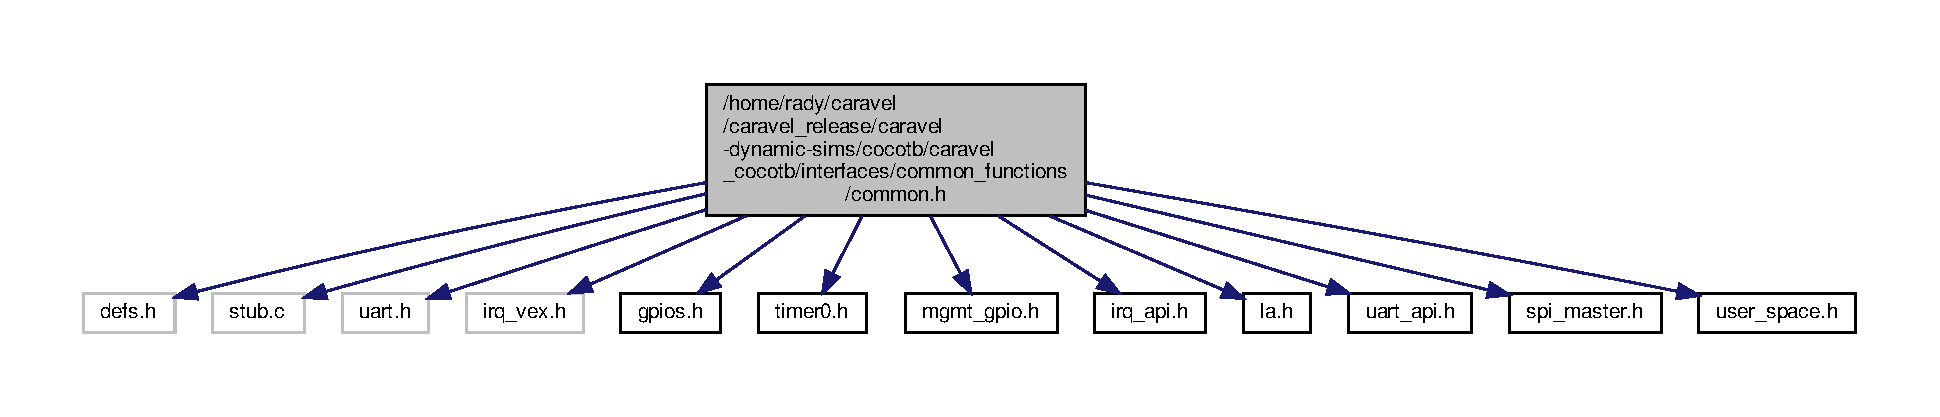
\includegraphics[width=350pt]{common_8h__incl}
\end{center}
\end{figure}
\subsection*{Functions}
\begin{DoxyCompactItemize}
\item 
void \hyperlink{common_8h_a08c5c91278b49a7e91696d5d526505e1}{enable\+Hk\+Spi} (bool is\+\_\+enable)
\item 
void \hyperlink{common_8h_a2693b1908ee935b4d73d7c8c4bb897e9}{dummy\+Delay} (int num)
\end{DoxyCompactItemize}


\subsection{Function Documentation}
\mbox{\Hypertarget{common_8h_a2693b1908ee935b4d73d7c8c4bb897e9}\label{common_8h_a2693b1908ee935b4d73d7c8c4bb897e9}} 
\index{common.\+h@{common.\+h}!dummy\+Delay@{dummy\+Delay}}
\index{dummy\+Delay@{dummy\+Delay}!common.\+h@{common.\+h}}
\subsubsection{\texorpdfstring{dummy\+Delay()}{dummyDelay()}}
{\footnotesize\ttfamily void dummy\+Delay (\begin{DoxyParamCaption}\item[{int}]{num }\end{DoxyParamCaption})}

Insert delay


\begin{DoxyParams}{Parameters}
{\em num} & number of delays steps. step is increment local variable and check it\textquotesingle{}s value \\
\hline
\end{DoxyParams}
\mbox{\Hypertarget{common_8h_a08c5c91278b49a7e91696d5d526505e1}\label{common_8h_a08c5c91278b49a7e91696d5d526505e1}} 
\index{common.\+h@{common.\+h}!enable\+Hk\+Spi@{enable\+Hk\+Spi}}
\index{enable\+Hk\+Spi@{enable\+Hk\+Spi}!common.\+h@{common.\+h}}
\subsubsection{\texorpdfstring{enable\+Hk\+Spi()}{enableHkSpi()}}
{\footnotesize\ttfamily void enable\+Hk\+Spi (\begin{DoxyParamCaption}\item[{bool}]{is\+\_\+enable }\end{DoxyParamCaption})}

Enable or disable the housekeeping S\+PI This function writes to the housekeeping disenable register inside the housekeeping \begin{DoxyNote}{Note}
When this register asserted housekeeping S\+PI can\textquotesingle{}t be used and G\+P\+I\+Os\mbox{[}3\mbox{]} which is C\+SB can be used as any other Caravel G\+P\+I\+Os
\end{DoxyNote}
\begin{DoxyWarning}{Warning}
By default the housekeeping S\+PI is enabled to use G\+P\+I\+Os\mbox{[}3\mbox{]} freely it should be disabled.
\end{DoxyWarning}

\begin{DoxyParams}{Parameters}
{\em is\+\_\+enable} & when 1 (true) housekeeping is active, 0 (false) housekeeping is disabled \\
\hline
\end{DoxyParams}

\hypertarget{gpios_8h}{}\section{/home/rady/caravel/caravel\+\_\+release/caravel-\/dynamic-\/sims/cocotb/caravel\+\_\+cocotb/interfaces/common\+\_\+functions/gpios.h File Reference}
\label{gpios_8h}\index{/home/rady/caravel/caravel\+\_\+release/caravel-\/dynamic-\/sims/cocotb/caravel\+\_\+cocotb/interfaces/common\+\_\+functions/gpios.\+h@{/home/rady/caravel/caravel\+\_\+release/caravel-\/dynamic-\/sims/cocotb/caravel\+\_\+cocotb/interfaces/common\+\_\+functions/gpios.\+h}}
This graph shows which files directly or indirectly include this file\+:\nopagebreak
\begin{figure}[H]
\begin{center}
\leavevmode
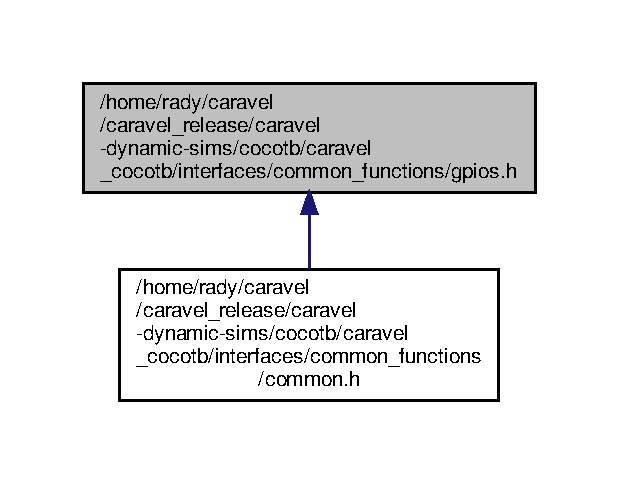
\includegraphics[width=297pt]{gpios_8h__dep__incl}
\end{center}
\end{figure}
\subsection*{Enumerations}
\begin{DoxyCompactItemize}
\item 
enum \hyperlink{gpios_8h_a620d533a2ccc5296d2f6c8b95bf89fe1}{gpio\+\_\+mode} 
\end{DoxyCompactItemize}
\subsection*{Functions}
\begin{DoxyCompactItemize}
\item 
void \hyperlink{gpios_8h_af288a525a946a5cb8265a07235cc0a89}{G\+P\+I\+Os\+\_\+configure\+All} (enum \hyperlink{gpios_8h_a620d533a2ccc5296d2f6c8b95bf89fe1}{gpio\+\_\+mode} config)
\item 
void \hyperlink{gpios_8h_aa2d753ef0720dd40c8cca9d386ccab85}{G\+P\+I\+Os\+\_\+load\+Configs} ()
\item 
void \hyperlink{gpios_8h_a7741f231d1f7f3ddd4c3e65e1623d29b}{G\+P\+I\+Os\+\_\+configure} (int gpio\+\_\+num, enum \hyperlink{gpios_8h_a620d533a2ccc5296d2f6c8b95bf89fe1}{gpio\+\_\+mode} config)
\item 
void \hyperlink{gpios_8h_a503d40479dae4e1d776f9a828da26e9c}{G\+P\+I\+Os\+\_\+write\+Low} (unsigned int data)
\item 
void \hyperlink{gpios_8h_a7839dcf1479c966ba9434fd3cafde145}{G\+P\+I\+Os\+\_\+write\+High} (unsigned int data)
\item 
void \hyperlink{gpios_8h_aa0bdfb4d673bf0f766c0883b914fc00c}{G\+P\+I\+Os\+\_\+write\+Low\+High} (long data)
\item 
unsigned int \hyperlink{gpios_8h_a38a69d74731490954747a059d9c7b3de}{G\+P\+I\+Os\+\_\+read\+High} ()
\item 
unsigned int \hyperlink{gpios_8h_a6e492397b64caf85c5a36ac0c8e1d00d}{G\+P\+I\+Os\+\_\+read\+Low} ()
\item 
void \hyperlink{gpios_8h_a196f858ea2a3307d453288e2426de274}{G\+P\+I\+Os\+\_\+wait\+Low} (unsigned int data)
\item 
void \hyperlink{gpios_8h_a5633f00a1a81df2ae81341ee04658ea6}{G\+P\+I\+Os\+\_\+wait\+High} (unsigned int data)
\item 
void \hyperlink{gpios_8h_a7eac3b1a8b68f8fef71169ca40a21742}{G\+P\+I\+Os\+\_\+wait\+Low\+With\+Mask} (unsigned int data, unsigned int mask)
\item 
void \hyperlink{gpios_8h_a83b74468a9ef251ca1da1fb5f0948869}{G\+P\+I\+Os\+\_\+wait\+High\+With\+Mask} (unsigned int data, unsigned int mask)
\end{DoxyCompactItemize}


\subsection{Enumeration Type Documentation}
\mbox{\Hypertarget{gpios_8h_a620d533a2ccc5296d2f6c8b95bf89fe1}\label{gpios_8h_a620d533a2ccc5296d2f6c8b95bf89fe1}} 
\index{gpios.\+h@{gpios.\+h}!gpio\+\_\+mode@{gpio\+\_\+mode}}
\index{gpio\+\_\+mode@{gpio\+\_\+mode}!gpios.\+h@{gpios.\+h}}
\subsubsection{\texorpdfstring{gpio\+\_\+mode}{gpio\_mode}}
{\footnotesize\ttfamily enum \hyperlink{gpios_8h_a620d533a2ccc5296d2f6c8b95bf89fe1}{gpio\+\_\+mode}}

G\+P\+I\+Os possible modes \hypertarget{user__space_8h_multi_row}{}
\tabulinesep=1mm
\begin{longtabu} spread 0pt [c]{*{2}{|X[-1]}|}
\caption{Enumerator gpio\+\_\+mode}\label{user__space_8h_multi_row}\\
\hline
\rowcolor{\tableheadbgcolor}\textbf{ name}&\textbf{ description }\\\cline{1-2}
\endfirsthead
\hline
\endfoot
\hline
\rowcolor{\tableheadbgcolor}\textbf{ name}&\textbf{ description }\\\cline{1-2}
\endhead
G\+P\+I\+O\+\_\+\+M\+O\+D\+E\+\_\+\+M\+G\+M\+T\+\_\+\+S\+T\+D\+\_\+\+I\+N\+P\+U\+T\+\_\+\+N\+O\+P\+U\+LL&Management input with no pull (floating is read as Z) \\\cline{1-2}
G\+P\+I\+O\+\_\+\+M\+O\+D\+E\+\_\+\+M\+G\+M\+T\+\_\+\+S\+T\+D\+\_\+\+I\+N\+P\+U\+T\+\_\+\+P\+U\+L\+L\+D\+O\+WN&Management input pull-\/down (floating is read as 0) \\\cline{1-2}
G\+P\+I\+O\+\_\+\+M\+O\+D\+E\+\_\+\+M\+G\+M\+T\+\_\+\+S\+T\+D\+\_\+\+I\+N\+P\+U\+T\+\_\+\+P\+U\+L\+L\+UP&Management input pull-\/up (floating is read as 1) \\\cline{1-2}
G\+P\+I\+O\+\_\+\+M\+O\+D\+E\+\_\+\+M\+G\+M\+T\+\_\+\+S\+T\+D\+\_\+\+O\+U\+T\+P\+UT&Management output \\\cline{1-2}
G\+P\+I\+O\+\_\+\+M\+O\+D\+E\+\_\+\+M\+G\+M\+T\+\_\+\+S\+T\+D\+\_\+\+B\+I\+D\+I\+R\+E\+C\+T\+I\+O\+N\+AL&Management bi-\/direction \\\cline{1-2}
G\+P\+I\+O\+\_\+\+M\+O\+D\+E\+\_\+\+M\+G\+M\+T\+\_\+\+S\+T\+D\+\_\+\+A\+N\+A\+L\+OG&Management Analog \\\cline{1-2}
G\+P\+I\+O\+\_\+\+M\+O\+D\+E\+\_\+\+U\+S\+E\+R\+\_\+\+S\+T\+D\+\_\+\+I\+N\+P\+U\+T\+\_\+\+N\+O\+P\+U\+LL&User input with no pull (floating is read as Z) \\\cline{1-2}
G\+P\+I\+O\+\_\+\+M\+O\+D\+E\+\_\+\+U\+S\+E\+R\+\_\+\+S\+T\+D\+\_\+\+I\+N\+P\+U\+T\+\_\+\+P\+U\+L\+L\+D\+O\+WN&User input pull-\/down (floating is read as 0) \\\cline{1-2}
G\+P\+I\+O\+\_\+\+M\+O\+D\+E\+\_\+\+U\+S\+E\+R\+\_\+\+S\+T\+D\+\_\+\+I\+N\+P\+U\+T\+\_\+\+P\+U\+L\+L\+UP&User input pull-\/up (floating is read as 1) \\\cline{1-2}
G\+P\+I\+O\+\_\+\+M\+O\+D\+E\+\_\+\+U\+S\+E\+R\+\_\+\+S\+T\+D\+\_\+\+O\+U\+T\+P\+UT&User output \\\cline{1-2}
G\+P\+I\+O\+\_\+\+M\+O\+D\+E\+\_\+\+U\+S\+E\+R\+\_\+\+S\+T\+D\+\_\+\+B\+I\+D\+I\+R\+E\+C\+T\+I\+O\+N\+AL&User bi-\/direction \\\cline{1-2}
G\+P\+I\+O\+\_\+\+M\+O\+D\+E\+\_\+\+U\+S\+E\+R\+\_\+\+S\+T\+D\+\_\+\+O\+U\+T\+\_\+\+M\+O\+N\+I\+T\+O\+R\+ED&User Monitor same as output \\\cline{1-2}
G\+P\+I\+O\+\_\+\+M\+O\+D\+E\+\_\+\+U\+S\+E\+R\+\_\+\+S\+T\+D\+\_\+\+A\+N\+A\+L\+OG&User Analog \\\cline{1-2}
\end{longtabu}


\subsection{Function Documentation}
\mbox{\Hypertarget{gpios_8h_a7741f231d1f7f3ddd4c3e65e1623d29b}\label{gpios_8h_a7741f231d1f7f3ddd4c3e65e1623d29b}} 
\index{gpios.\+h@{gpios.\+h}!G\+P\+I\+Os\+\_\+configure@{G\+P\+I\+Os\+\_\+configure}}
\index{G\+P\+I\+Os\+\_\+configure@{G\+P\+I\+Os\+\_\+configure}!gpios.\+h@{gpios.\+h}}
\subsubsection{\texorpdfstring{G\+P\+I\+Os\+\_\+configure()}{GPIOs\_configure()}}
{\footnotesize\ttfamily void G\+P\+I\+Os\+\_\+configure (\begin{DoxyParamCaption}\item[{int}]{gpio\+\_\+num,  }\item[{enum \hyperlink{gpios_8h_a620d533a2ccc5296d2f6c8b95bf89fe1}{gpio\+\_\+mode}}]{config }\end{DoxyParamCaption})}

Configure one G\+P\+IO with the input config


\begin{DoxyParams}{Parameters}
{\em config} & is configuration of type gpio\+\_\+mode \\
\hline
{\em gpio\+\_\+num} & is G\+P\+IO number it can have values from 0 to 37\\
\hline
\end{DoxyParams}
\begin{DoxyNote}{Note}
These configurations will not be change the G\+P\+I\+Os modes until calling \hyperlink{gpios_8h_aa2d753ef0720dd40c8cca9d386ccab85}{G\+P\+I\+Os\+\_\+load\+Configs()} 
\end{DoxyNote}
\mbox{\Hypertarget{gpios_8h_af288a525a946a5cb8265a07235cc0a89}\label{gpios_8h_af288a525a946a5cb8265a07235cc0a89}} 
\index{gpios.\+h@{gpios.\+h}!G\+P\+I\+Os\+\_\+configure\+All@{G\+P\+I\+Os\+\_\+configure\+All}}
\index{G\+P\+I\+Os\+\_\+configure\+All@{G\+P\+I\+Os\+\_\+configure\+All}!gpios.\+h@{gpios.\+h}}
\subsubsection{\texorpdfstring{G\+P\+I\+Os\+\_\+configure\+All()}{GPIOs\_configureAll()}}
{\footnotesize\ttfamily void G\+P\+I\+Os\+\_\+configure\+All (\begin{DoxyParamCaption}\item[{enum \hyperlink{gpios_8h_a620d533a2ccc5296d2f6c8b95bf89fe1}{gpio\+\_\+mode}}]{config }\end{DoxyParamCaption})}

Configure all G\+P\+I\+Os with the config


\begin{DoxyParams}{Parameters}
{\em config} & is configuration of type gpio\+\_\+mode\\
\hline
\end{DoxyParams}
\begin{DoxyNote}{Note}
These configurations will not be change the G\+P\+I\+Os modes until calling \hyperlink{gpios_8h_aa2d753ef0720dd40c8cca9d386ccab85}{G\+P\+I\+Os\+\_\+load\+Configs()} 
\end{DoxyNote}
\mbox{\Hypertarget{gpios_8h_aa2d753ef0720dd40c8cca9d386ccab85}\label{gpios_8h_aa2d753ef0720dd40c8cca9d386ccab85}} 
\index{gpios.\+h@{gpios.\+h}!G\+P\+I\+Os\+\_\+load\+Configs@{G\+P\+I\+Os\+\_\+load\+Configs}}
\index{G\+P\+I\+Os\+\_\+load\+Configs@{G\+P\+I\+Os\+\_\+load\+Configs}!gpios.\+h@{gpios.\+h}}
\subsubsection{\texorpdfstring{G\+P\+I\+Os\+\_\+load\+Configs()}{GPIOs\_loadConfigs()}}
{\footnotesize\ttfamily void G\+P\+I\+Os\+\_\+load\+Configs (\begin{DoxyParamCaption}{ }\end{DoxyParamCaption})}

Load the configurations changes to the G\+P\+I\+Os \mbox{\Hypertarget{gpios_8h_a38a69d74731490954747a059d9c7b3de}\label{gpios_8h_a38a69d74731490954747a059d9c7b3de}} 
\index{gpios.\+h@{gpios.\+h}!G\+P\+I\+Os\+\_\+read\+High@{G\+P\+I\+Os\+\_\+read\+High}}
\index{G\+P\+I\+Os\+\_\+read\+High@{G\+P\+I\+Os\+\_\+read\+High}!gpios.\+h@{gpios.\+h}}
\subsubsection{\texorpdfstring{G\+P\+I\+Os\+\_\+read\+High()}{GPIOs\_readHigh()}}
{\footnotesize\ttfamily unsigned int G\+P\+I\+Os\+\_\+read\+High (\begin{DoxyParamCaption}{ }\end{DoxyParamCaption})}

Read the highest 6 G\+P\+I\+Os G\+P\+I\+OS\mbox{[}37\+:32\mbox{]} \begin{DoxyNote}{Note}
For Reading value from the G\+P\+I\+Os, the G\+P\+IO should be configured as management input. otherwise 0 would be read 
\end{DoxyNote}
\mbox{\Hypertarget{gpios_8h_a6e492397b64caf85c5a36ac0c8e1d00d}\label{gpios_8h_a6e492397b64caf85c5a36ac0c8e1d00d}} 
\index{gpios.\+h@{gpios.\+h}!G\+P\+I\+Os\+\_\+read\+Low@{G\+P\+I\+Os\+\_\+read\+Low}}
\index{G\+P\+I\+Os\+\_\+read\+Low@{G\+P\+I\+Os\+\_\+read\+Low}!gpios.\+h@{gpios.\+h}}
\subsubsection{\texorpdfstring{G\+P\+I\+Os\+\_\+read\+Low()}{GPIOs\_readLow()}}
{\footnotesize\ttfamily unsigned int G\+P\+I\+Os\+\_\+read\+Low (\begin{DoxyParamCaption}{ }\end{DoxyParamCaption})}

Read low 32 G\+P\+I\+Os G\+P\+I\+OS\mbox{[}31\+:0\mbox{]} \begin{DoxyNote}{Note}
For Reading value from the G\+P\+I\+Os, the G\+P\+IO should be configured as management input. otherwise 0 would be read 
\end{DoxyNote}
\mbox{\Hypertarget{gpios_8h_a5633f00a1a81df2ae81341ee04658ea6}\label{gpios_8h_a5633f00a1a81df2ae81341ee04658ea6}} 
\index{gpios.\+h@{gpios.\+h}!G\+P\+I\+Os\+\_\+wait\+High@{G\+P\+I\+Os\+\_\+wait\+High}}
\index{G\+P\+I\+Os\+\_\+wait\+High@{G\+P\+I\+Os\+\_\+wait\+High}!gpios.\+h@{gpios.\+h}}
\subsubsection{\texorpdfstring{G\+P\+I\+Os\+\_\+wait\+High()}{GPIOs\_waitHigh()}}
{\footnotesize\ttfamily void G\+P\+I\+Os\+\_\+wait\+High (\begin{DoxyParamCaption}\item[{unsigned int}]{data }\end{DoxyParamCaption})}

wait over the highest 6 G\+P\+I\+Os to equal the data passed \begin{DoxyNote}{Note}
For writing by this function to be seen at the G\+P\+IO the G\+P\+IO has to be configured as management output
\end{DoxyNote}

\begin{DoxyParams}{Parameters}
{\em data} & is the data that should wait until sent to the G\+P\+I\+Os\\
\hline
\end{DoxyParams}
Examples\+: \begin{DoxyItemize}
\item 
\begin{DoxyCode}
\hyperlink{gpios_8h_a5633f00a1a81df2ae81341ee04658ea6}{GPIOs\_waitHigh}(0x1); \textcolor{comment}{// function would return only when GPIO [32]==1 and rest of 5 GPIOs = 0 
       }
\end{DoxyCode}
 \item 
\begin{DoxyCode}
\hyperlink{gpios_8h_a5633f00a1a81df2ae81341ee04658ea6}{GPIOs\_waitHigh}(0x5); \textcolor{comment}{// function would return only when GPIO [32]==1 and GPIO [34]==1 and
       rest of 4 GPIOs = 0 }
\end{DoxyCode}
 \end{DoxyItemize}
\mbox{\Hypertarget{gpios_8h_a83b74468a9ef251ca1da1fb5f0948869}\label{gpios_8h_a83b74468a9ef251ca1da1fb5f0948869}} 
\index{gpios.\+h@{gpios.\+h}!G\+P\+I\+Os\+\_\+wait\+High\+With\+Mask@{G\+P\+I\+Os\+\_\+wait\+High\+With\+Mask}}
\index{G\+P\+I\+Os\+\_\+wait\+High\+With\+Mask@{G\+P\+I\+Os\+\_\+wait\+High\+With\+Mask}!gpios.\+h@{gpios.\+h}}
\subsubsection{\texorpdfstring{G\+P\+I\+Os\+\_\+wait\+High\+With\+Mask()}{GPIOs\_waitHighWithMask()}}
{\footnotesize\ttfamily void G\+P\+I\+Os\+\_\+wait\+High\+With\+Mask (\begin{DoxyParamCaption}\item[{unsigned int}]{data,  }\item[{unsigned int}]{mask }\end{DoxyParamCaption})}

wait over the masked highest 6 G\+P\+I\+Os to equal the data passed \begin{DoxyNote}{Note}
For writing by this function to be seen at the G\+P\+IO the G\+P\+IO has to be configured as management output
\end{DoxyNote}

\begin{DoxyParams}{Parameters}
{\em data} & is the data that should wait until sent to the G\+P\+I\+Os \\
\hline
{\em mask} & mask over the each G\+P\+IO if the mask value is 0 the this G\+P\+IO value are ignored\\
\hline
\end{DoxyParams}
Examples\+: \begin{DoxyItemize}
\item 
\begin{DoxyCode}
\hyperlink{gpios_8h_a83b74468a9ef251ca1da1fb5f0948869}{GPIOs\_waitHighWithMask}(0x1,0xF); \textcolor{comment}{// function would return only when GPIO [32]==1 and
       GPIO [35:33]==0 and don't care about the rest of GPIOs  }
\end{DoxyCode}
 \item 
\begin{DoxyCode}
\hyperlink{gpios_8h_a83b74468a9ef251ca1da1fb5f0948869}{GPIOs\_waitHighWithMask}(0x5,0x7); \textcolor{comment}{// function would return only when GPIO [32]==1 and
       GPIO [34]==1 and GPIO [33]==0 and don't care about the rest of GPIOs }
\end{DoxyCode}
 \end{DoxyItemize}
\mbox{\Hypertarget{gpios_8h_a196f858ea2a3307d453288e2426de274}\label{gpios_8h_a196f858ea2a3307d453288e2426de274}} 
\index{gpios.\+h@{gpios.\+h}!G\+P\+I\+Os\+\_\+wait\+Low@{G\+P\+I\+Os\+\_\+wait\+Low}}
\index{G\+P\+I\+Os\+\_\+wait\+Low@{G\+P\+I\+Os\+\_\+wait\+Low}!gpios.\+h@{gpios.\+h}}
\subsubsection{\texorpdfstring{G\+P\+I\+Os\+\_\+wait\+Low()}{GPIOs\_waitLow()}}
{\footnotesize\ttfamily void G\+P\+I\+Os\+\_\+wait\+Low (\begin{DoxyParamCaption}\item[{unsigned int}]{data }\end{DoxyParamCaption})}

wait over the lowest 32 G\+P\+I\+Osto equal the data passed \begin{DoxyNote}{Note}
For writing by this function to be seen at the G\+P\+IO the G\+P\+IO has to be configured as management output
\end{DoxyNote}

\begin{DoxyParams}{Parameters}
{\em data} & is the data that should wait until sent to the G\+P\+I\+Os\\
\hline
\end{DoxyParams}
Examples\+: \begin{DoxyItemize}
\item 
\begin{DoxyCode}
\hyperlink{gpios_8h_a196f858ea2a3307d453288e2426de274}{GPIOs\_waitLow}(0x1); \textcolor{comment}{// function would return only when GPIO [0]==1 and rest of 31 GPIOs= 0  }
\end{DoxyCode}
 \item 
\begin{DoxyCode}
\hyperlink{gpios_8h_a196f858ea2a3307d453288e2426de274}{GPIOs\_waitLow}(0x5); \textcolor{comment}{// function would return only when GPIO [0]==1 and GPIO [3]==1 and rest of
       30 GPIOs = 0 }
\end{DoxyCode}
 \end{DoxyItemize}
\mbox{\Hypertarget{gpios_8h_a7eac3b1a8b68f8fef71169ca40a21742}\label{gpios_8h_a7eac3b1a8b68f8fef71169ca40a21742}} 
\index{gpios.\+h@{gpios.\+h}!G\+P\+I\+Os\+\_\+wait\+Low\+With\+Mask@{G\+P\+I\+Os\+\_\+wait\+Low\+With\+Mask}}
\index{G\+P\+I\+Os\+\_\+wait\+Low\+With\+Mask@{G\+P\+I\+Os\+\_\+wait\+Low\+With\+Mask}!gpios.\+h@{gpios.\+h}}
\subsubsection{\texorpdfstring{G\+P\+I\+Os\+\_\+wait\+Low\+With\+Mask()}{GPIOs\_waitLowWithMask()}}
{\footnotesize\ttfamily void G\+P\+I\+Os\+\_\+wait\+Low\+With\+Mask (\begin{DoxyParamCaption}\item[{unsigned int}]{data,  }\item[{unsigned int}]{mask }\end{DoxyParamCaption})}

wait over the masked lowest 32 G\+P\+I\+Os to equal the data passed \begin{DoxyNote}{Note}
For writing by this function to be seen at the G\+P\+IO the G\+P\+IO has to be configured as management output
\end{DoxyNote}

\begin{DoxyParams}{Parameters}
{\em data} & is the data that should wait until sent to the G\+P\+I\+Os \\
\hline
{\em mask} & mask over the each G\+P\+IO if the mask value is 0 the this G\+P\+IO value are ignored\\
\hline
\end{DoxyParams}
Examples\+: \begin{DoxyItemize}
\item 
\begin{DoxyCode}
\hyperlink{gpios_8h_a7eac3b1a8b68f8fef71169ca40a21742}{GPIOs\_waitLowWithMask}(0x1,0xF); \textcolor{comment}{// function would return only when GPIO [0]==1 and
       GPIO [3:1]==0 and don't care about the rest of GPIOs  }
\end{DoxyCode}
 \item 
\begin{DoxyCode}
\hyperlink{gpios_8h_a7eac3b1a8b68f8fef71169ca40a21742}{GPIOs\_waitLowWithMask}(0x5,0x7); \textcolor{comment}{// function would return only when GPIO [0]==1 and
       GPIO [3]==1 and GPIO [2]==0 and don't care about the rest of GPIOs }
\end{DoxyCode}
 \end{DoxyItemize}
\mbox{\Hypertarget{gpios_8h_a7839dcf1479c966ba9434fd3cafde145}\label{gpios_8h_a7839dcf1479c966ba9434fd3cafde145}} 
\index{gpios.\+h@{gpios.\+h}!G\+P\+I\+Os\+\_\+write\+High@{G\+P\+I\+Os\+\_\+write\+High}}
\index{G\+P\+I\+Os\+\_\+write\+High@{G\+P\+I\+Os\+\_\+write\+High}!gpios.\+h@{gpios.\+h}}
\subsubsection{\texorpdfstring{G\+P\+I\+Os\+\_\+write\+High()}{GPIOs\_writeHigh()}}
{\footnotesize\ttfamily void G\+P\+I\+Os\+\_\+write\+High (\begin{DoxyParamCaption}\item[{unsigned int}]{data }\end{DoxyParamCaption})}

Write to the highest 6 G\+P\+I\+Os G\+P\+I\+OS\mbox{[}37\+:32\mbox{]} \begin{DoxyNote}{Note}
For writing by this function to be seen at the G\+P\+IO the G\+P\+IO has to be configured as management output
\end{DoxyNote}

\begin{DoxyParams}{Parameters}
{\em data} & is the data sent to the G\+P\+I\+Os\\
\hline
\end{DoxyParams}
Examples\+: \begin{DoxyItemize}
\item 
\begin{DoxyCode}
\hyperlink{gpios_8h_a7839dcf1479c966ba9434fd3cafde145}{GPIOs\_writeHigh}(0x1); \textcolor{comment}{// write 1 to GPIO [32] and write 0 in the remaining 5 GPIOs}
\end{DoxyCode}
 \item 
\begin{DoxyCode}
\hyperlink{gpios_8h_a7839dcf1479c966ba9434fd3cafde145}{GPIOs\_writeHigh}(0x5); \textcolor{comment}{// write 1 to GPIO [32] and 34 and write 0 in the remaining 4 GPIOs}
\end{DoxyCode}
 \end{DoxyItemize}
\mbox{\Hypertarget{gpios_8h_a503d40479dae4e1d776f9a828da26e9c}\label{gpios_8h_a503d40479dae4e1d776f9a828da26e9c}} 
\index{gpios.\+h@{gpios.\+h}!G\+P\+I\+Os\+\_\+write\+Low@{G\+P\+I\+Os\+\_\+write\+Low}}
\index{G\+P\+I\+Os\+\_\+write\+Low@{G\+P\+I\+Os\+\_\+write\+Low}!gpios.\+h@{gpios.\+h}}
\subsubsection{\texorpdfstring{G\+P\+I\+Os\+\_\+write\+Low()}{GPIOs\_writeLow()}}
{\footnotesize\ttfamily void G\+P\+I\+Os\+\_\+write\+Low (\begin{DoxyParamCaption}\item[{unsigned int}]{data }\end{DoxyParamCaption})}

Write to the low 32 G\+P\+I\+Os G\+P\+I\+OS\mbox{[}31\+:0\mbox{]} \begin{DoxyNote}{Note}
For writing by this function to be seen at the G\+P\+IO the G\+P\+IO has to be configured as management output
\end{DoxyNote}

\begin{DoxyParams}{Parameters}
{\em data} & is the data sent to the G\+P\+I\+Os\\
\hline
\end{DoxyParams}
Examples\+: \begin{DoxyItemize}
\item 
\begin{DoxyCode}
\hyperlink{gpios_8h_a503d40479dae4e1d776f9a828da26e9c}{GPIOs\_writeLow}(0x1); \textcolor{comment}{// write 1 to GPIO [0] and write 0 in the remaining 31 GPIOs }
\end{DoxyCode}
 \item 
\begin{DoxyCode}
\hyperlink{gpios_8h_a503d40479dae4e1d776f9a828da26e9c}{GPIOs\_writeLow}(0x5); \textcolor{comment}{// write 1 to GPIO [0] and GPIO [3] and write 0 in the remaining 30
       GPIOs}
\end{DoxyCode}
 \end{DoxyItemize}
\mbox{\Hypertarget{gpios_8h_aa0bdfb4d673bf0f766c0883b914fc00c}\label{gpios_8h_aa0bdfb4d673bf0f766c0883b914fc00c}} 
\index{gpios.\+h@{gpios.\+h}!G\+P\+I\+Os\+\_\+write\+Low\+High@{G\+P\+I\+Os\+\_\+write\+Low\+High}}
\index{G\+P\+I\+Os\+\_\+write\+Low\+High@{G\+P\+I\+Os\+\_\+write\+Low\+High}!gpios.\+h@{gpios.\+h}}
\subsubsection{\texorpdfstring{G\+P\+I\+Os\+\_\+write\+Low\+High()}{GPIOs\_writeLowHigh()}}
{\footnotesize\ttfamily void G\+P\+I\+Os\+\_\+write\+Low\+High (\begin{DoxyParamCaption}\item[{long}]{data }\end{DoxyParamCaption})}

Write to the 38 G\+P\+I\+Os G\+P\+I\+OS\mbox{[}37\+:0\mbox{]} \begin{DoxyNote}{Note}
For writing by this function to be seen at the G\+P\+IO the G\+P\+IO has to be configured as management output
\end{DoxyNote}

\begin{DoxyParams}{Parameters}
{\em data} & is the data sent to the G\+P\+I\+Os\\
\hline
\end{DoxyParams}
Examples\+: \begin{DoxyItemize}
\item 
\begin{DoxyCode}
\hyperlink{gpios_8h_aa0bdfb4d673bf0f766c0883b914fc00c}{GPIOs\_writeLowHigh}(0x1); \textcolor{comment}{// write 1 to GPIO [0] and write 0 in the remaining 37 GPIOs }
\end{DoxyCode}
 \item 
\begin{DoxyCode}
\hyperlink{gpios_8h_aa0bdfb4d673bf0f766c0883b914fc00c}{GPIOs\_writeLowHigh}(0x5); \textcolor{comment}{// write 1 to GPIO [0] and GPIO [3] and write 0 in the remaining
       36 GPIOs}
\end{DoxyCode}
 \item 
\begin{DoxyCode}
\hyperlink{gpios_8h_aa0bdfb4d673bf0f766c0883b914fc00c}{GPIOs\_writeLowHigh}(0x100000000); \textcolor{comment}{// write 1 to GPIO [32] and write 0 in the remaining 36
       GPIOs}
\end{DoxyCode}
\end{DoxyItemize}
\begin{DoxyRefDesc}{Todo}
\item[\hyperlink{todo__todo000001}{Todo}]verify this function \end{DoxyRefDesc}

\hypertarget{irq__api_8h}{}\section{/home/rady/caravel/caravel\+\_\+release/caravel-\/dynamic-\/sims/cocotb/caravel\+\_\+cocotb/interfaces/common\+\_\+functions/irq\+\_\+api.h File Reference}
\label{irq__api_8h}\index{/home/rady/caravel/caravel\+\_\+release/caravel-\/dynamic-\/sims/cocotb/caravel\+\_\+cocotb/interfaces/common\+\_\+functions/irq\+\_\+api.\+h@{/home/rady/caravel/caravel\+\_\+release/caravel-\/dynamic-\/sims/cocotb/caravel\+\_\+cocotb/interfaces/common\+\_\+functions/irq\+\_\+api.\+h}}
This graph shows which files directly or indirectly include this file\+:\nopagebreak
\begin{figure}[H]
\begin{center}
\leavevmode
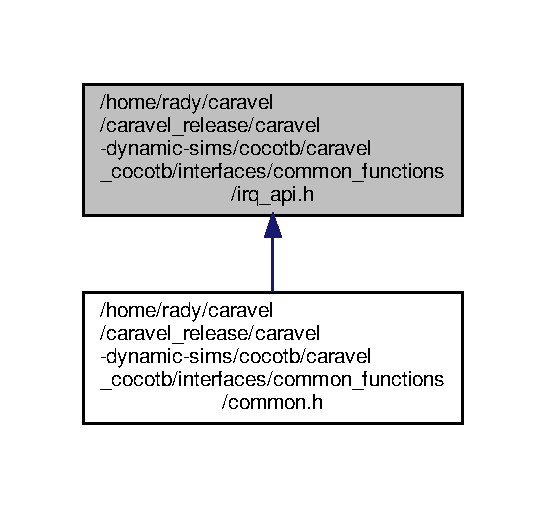
\includegraphics[width=262pt]{irq__api_8h__dep__incl}
\end{center}
\end{figure}
\subsection*{Functions}
\begin{DoxyCompactItemize}
\item 
void \hyperlink{irq__api_8h_a33f86b77b6c05de0aa9f8de0f1121876}{I\+R\+Q\+\_\+enable\+External1} (bool is\+\_\+enable)
\item 
void \hyperlink{irq__api_8h_ad7c5b62cb6e19b449ccf6711d31b8b35}{I\+R\+Q\+\_\+enable\+External2} (bool is\+\_\+enable)
\item 
void \hyperlink{irq__api_8h_a7c18bd8cbddb3e33141c99b3d02663b8}{I\+R\+Q\+\_\+enable\+User0} (bool is\+\_\+enable)
\item 
void \hyperlink{irq__api_8h_ac8b85a0ff4da956f253da5bb1a359a8f}{I\+R\+Q\+\_\+enable\+User1} (bool is\+\_\+enable)
\item 
void \hyperlink{irq__api_8h_aa7e7badb5afb49dd8a1e855b676da84a}{I\+R\+Q\+\_\+enable\+User2} (bool is\+\_\+enable)
\item 
void \hyperlink{irq__api_8h_a2bf7c0011bc8a27bada789eabbb08e6c}{I\+R\+Q\+\_\+enable\+Timer} (bool is\+\_\+enable)
\item 
void \hyperlink{irq__api_8h_a4f13c9b7d087417cdfe2406fee2d4b62}{I\+R\+Q\+\_\+enable\+Uart\+Tx} (bool is\+\_\+enable)
\item 
void \hyperlink{irq__api_8h_a4cda68c6fb315ebcde31cfc54170e307}{I\+R\+Q\+\_\+enable\+Uart\+Rx} (bool is\+\_\+enable)
\item 
void \hyperlink{irq__api_8h_ad05bfdede736222a7348204bb84937a4}{I\+R\+Q\+\_\+hk\+Spi} (bool is\+\_\+enable)
\end{DoxyCompactItemize}


\subsection{Function Documentation}
\mbox{\Hypertarget{irq__api_8h_a33f86b77b6c05de0aa9f8de0f1121876}\label{irq__api_8h_a33f86b77b6c05de0aa9f8de0f1121876}} 
\index{irq\+\_\+api.\+h@{irq\+\_\+api.\+h}!I\+R\+Q\+\_\+enable\+External1@{I\+R\+Q\+\_\+enable\+External1}}
\index{I\+R\+Q\+\_\+enable\+External1@{I\+R\+Q\+\_\+enable\+External1}!irq\+\_\+api.\+h@{irq\+\_\+api.\+h}}
\subsubsection{\texorpdfstring{I\+R\+Q\+\_\+enable\+External1()}{IRQ\_enableExternal1()}}
{\footnotesize\ttfamily void I\+R\+Q\+\_\+enable\+External1 (\begin{DoxyParamCaption}\item[{bool}]{is\+\_\+enable }\end{DoxyParamCaption})}

Enable or disable external1 interrupt G\+P\+IO\mbox{[}7\mbox{]}


\begin{DoxyParams}{Parameters}
{\em is\+\_\+enable} & when 1 (true) interrupt is active and firmware would detect if happened, 0 (false) interrupt is disabled and firmware would not detect if happened \\
\hline
\end{DoxyParams}
\mbox{\Hypertarget{irq__api_8h_ad7c5b62cb6e19b449ccf6711d31b8b35}\label{irq__api_8h_ad7c5b62cb6e19b449ccf6711d31b8b35}} 
\index{irq\+\_\+api.\+h@{irq\+\_\+api.\+h}!I\+R\+Q\+\_\+enable\+External2@{I\+R\+Q\+\_\+enable\+External2}}
\index{I\+R\+Q\+\_\+enable\+External2@{I\+R\+Q\+\_\+enable\+External2}!irq\+\_\+api.\+h@{irq\+\_\+api.\+h}}
\subsubsection{\texorpdfstring{I\+R\+Q\+\_\+enable\+External2()}{IRQ\_enableExternal2()}}
{\footnotesize\ttfamily void I\+R\+Q\+\_\+enable\+External2 (\begin{DoxyParamCaption}\item[{bool}]{is\+\_\+enable }\end{DoxyParamCaption})}

Enable or disable external2 interrupt G\+P\+IO\mbox{[}12\mbox{]}


\begin{DoxyParams}{Parameters}
{\em is\+\_\+enable} & when 1 (true) interrupt is active and firmware would detect if happened, 0 (false) interrupt is disabled and firmware would not detect if happened \\
\hline
\end{DoxyParams}
\mbox{\Hypertarget{irq__api_8h_a2bf7c0011bc8a27bada789eabbb08e6c}\label{irq__api_8h_a2bf7c0011bc8a27bada789eabbb08e6c}} 
\index{irq\+\_\+api.\+h@{irq\+\_\+api.\+h}!I\+R\+Q\+\_\+enable\+Timer@{I\+R\+Q\+\_\+enable\+Timer}}
\index{I\+R\+Q\+\_\+enable\+Timer@{I\+R\+Q\+\_\+enable\+Timer}!irq\+\_\+api.\+h@{irq\+\_\+api.\+h}}
\subsubsection{\texorpdfstring{I\+R\+Q\+\_\+enable\+Timer()}{IRQ\_enableTimer()}}
{\footnotesize\ttfamily void I\+R\+Q\+\_\+enable\+Timer (\begin{DoxyParamCaption}\item[{bool}]{is\+\_\+enable }\end{DoxyParamCaption})}

Enable or disable timer0 interrupt


\begin{DoxyParams}{Parameters}
{\em is\+\_\+enable} & when 1 (true) interrupt is active and firmware would detect if happened, 0 (false) interrupt is disabled and firmware would not detect if happened \\
\hline
\end{DoxyParams}
\mbox{\Hypertarget{irq__api_8h_a4cda68c6fb315ebcde31cfc54170e307}\label{irq__api_8h_a4cda68c6fb315ebcde31cfc54170e307}} 
\index{irq\+\_\+api.\+h@{irq\+\_\+api.\+h}!I\+R\+Q\+\_\+enable\+Uart\+Rx@{I\+R\+Q\+\_\+enable\+Uart\+Rx}}
\index{I\+R\+Q\+\_\+enable\+Uart\+Rx@{I\+R\+Q\+\_\+enable\+Uart\+Rx}!irq\+\_\+api.\+h@{irq\+\_\+api.\+h}}
\subsubsection{\texorpdfstring{I\+R\+Q\+\_\+enable\+Uart\+Rx()}{IRQ\_enableUartRx()}}
{\footnotesize\ttfamily void I\+R\+Q\+\_\+enable\+Uart\+Rx (\begin{DoxyParamCaption}\item[{bool}]{is\+\_\+enable }\end{DoxyParamCaption})}

Enable or disable U\+A\+RT rx interrupt


\begin{DoxyParams}{Parameters}
{\em is\+\_\+enable} & when 1 (true) interrupt is active and firmware would detect if happened, 0 (false) interrupt is disabled and firmware would not detect if happened \\
\hline
\end{DoxyParams}
\mbox{\Hypertarget{irq__api_8h_a4f13c9b7d087417cdfe2406fee2d4b62}\label{irq__api_8h_a4f13c9b7d087417cdfe2406fee2d4b62}} 
\index{irq\+\_\+api.\+h@{irq\+\_\+api.\+h}!I\+R\+Q\+\_\+enable\+Uart\+Tx@{I\+R\+Q\+\_\+enable\+Uart\+Tx}}
\index{I\+R\+Q\+\_\+enable\+Uart\+Tx@{I\+R\+Q\+\_\+enable\+Uart\+Tx}!irq\+\_\+api.\+h@{irq\+\_\+api.\+h}}
\subsubsection{\texorpdfstring{I\+R\+Q\+\_\+enable\+Uart\+Tx()}{IRQ\_enableUartTx()}}
{\footnotesize\ttfamily void I\+R\+Q\+\_\+enable\+Uart\+Tx (\begin{DoxyParamCaption}\item[{bool}]{is\+\_\+enable }\end{DoxyParamCaption})}

Enable or disable U\+A\+RT tx interrupt


\begin{DoxyParams}{Parameters}
{\em is\+\_\+enable} & when 1 (true) interrupt is active and firmware would detect if happened, 0 (false) interrupt is disabled and firmware would not detect if happened \\
\hline
\end{DoxyParams}
\mbox{\Hypertarget{irq__api_8h_a7c18bd8cbddb3e33141c99b3d02663b8}\label{irq__api_8h_a7c18bd8cbddb3e33141c99b3d02663b8}} 
\index{irq\+\_\+api.\+h@{irq\+\_\+api.\+h}!I\+R\+Q\+\_\+enable\+User0@{I\+R\+Q\+\_\+enable\+User0}}
\index{I\+R\+Q\+\_\+enable\+User0@{I\+R\+Q\+\_\+enable\+User0}!irq\+\_\+api.\+h@{irq\+\_\+api.\+h}}
\subsubsection{\texorpdfstring{I\+R\+Q\+\_\+enable\+User0()}{IRQ\_enableUser0()}}
{\footnotesize\ttfamily void I\+R\+Q\+\_\+enable\+User0 (\begin{DoxyParamCaption}\item[{bool}]{is\+\_\+enable }\end{DoxyParamCaption})}

Enable or disable user0 interrupt


\begin{DoxyParams}{Parameters}
{\em is\+\_\+enable} & when 1 (true) interrupt is active and firmware would detect if happened, 0 (false) interrupt is disabled and firmware would not detect if happened \\
\hline
\end{DoxyParams}
\mbox{\Hypertarget{irq__api_8h_ac8b85a0ff4da956f253da5bb1a359a8f}\label{irq__api_8h_ac8b85a0ff4da956f253da5bb1a359a8f}} 
\index{irq\+\_\+api.\+h@{irq\+\_\+api.\+h}!I\+R\+Q\+\_\+enable\+User1@{I\+R\+Q\+\_\+enable\+User1}}
\index{I\+R\+Q\+\_\+enable\+User1@{I\+R\+Q\+\_\+enable\+User1}!irq\+\_\+api.\+h@{irq\+\_\+api.\+h}}
\subsubsection{\texorpdfstring{I\+R\+Q\+\_\+enable\+User1()}{IRQ\_enableUser1()}}
{\footnotesize\ttfamily void I\+R\+Q\+\_\+enable\+User1 (\begin{DoxyParamCaption}\item[{bool}]{is\+\_\+enable }\end{DoxyParamCaption})}

Enable or disable user1 interrupt


\begin{DoxyParams}{Parameters}
{\em is\+\_\+enable} & when 1 (true) interrupt is active and firmware would detect if happened, 0 (false) interrupt is disabled and firmware would not detect if happened \\
\hline
\end{DoxyParams}
\mbox{\Hypertarget{irq__api_8h_aa7e7badb5afb49dd8a1e855b676da84a}\label{irq__api_8h_aa7e7badb5afb49dd8a1e855b676da84a}} 
\index{irq\+\_\+api.\+h@{irq\+\_\+api.\+h}!I\+R\+Q\+\_\+enable\+User2@{I\+R\+Q\+\_\+enable\+User2}}
\index{I\+R\+Q\+\_\+enable\+User2@{I\+R\+Q\+\_\+enable\+User2}!irq\+\_\+api.\+h@{irq\+\_\+api.\+h}}
\subsubsection{\texorpdfstring{I\+R\+Q\+\_\+enable\+User2()}{IRQ\_enableUser2()}}
{\footnotesize\ttfamily void I\+R\+Q\+\_\+enable\+User2 (\begin{DoxyParamCaption}\item[{bool}]{is\+\_\+enable }\end{DoxyParamCaption})}

Enable or disable user1 interrupt


\begin{DoxyParams}{Parameters}
{\em is\+\_\+enable} & when 1 (true) interrupt is active and firmware would detect if happened, 0 (false) interrupt is disabled and firmware would not detect if happened \\
\hline
\end{DoxyParams}
\mbox{\Hypertarget{irq__api_8h_ad05bfdede736222a7348204bb84937a4}\label{irq__api_8h_ad05bfdede736222a7348204bb84937a4}} 
\index{irq\+\_\+api.\+h@{irq\+\_\+api.\+h}!I\+R\+Q\+\_\+hk\+Spi@{I\+R\+Q\+\_\+hk\+Spi}}
\index{I\+R\+Q\+\_\+hk\+Spi@{I\+R\+Q\+\_\+hk\+Spi}!irq\+\_\+api.\+h@{irq\+\_\+api.\+h}}
\subsubsection{\texorpdfstring{I\+R\+Q\+\_\+hk\+Spi()}{IRQ\_hkSpi()}}
{\footnotesize\ttfamily void I\+R\+Q\+\_\+hk\+Spi (\begin{DoxyParamCaption}\item[{bool}]{is\+\_\+enable }\end{DoxyParamCaption})}

Enable or disable S\+PI interrupt


\begin{DoxyParams}{Parameters}
{\em is\+\_\+enable} & when 1 (true) interrupt is active and firmware would detect if happened, 0 (false) interrupt is disabled and firmware would not detect if happened \\
\hline
\end{DoxyParams}

\hypertarget{la_8h}{}\section{/home/rady/caravel/caravel\+\_\+release/caravel-\/dynamic-\/sims/cocotb/caravel\+\_\+cocotb/interfaces/common\+\_\+functions/la.h File Reference}
\label{la_8h}\index{/home/rady/caravel/caravel\+\_\+release/caravel-\/dynamic-\/sims/cocotb/caravel\+\_\+cocotb/interfaces/common\+\_\+functions/la.\+h@{/home/rady/caravel/caravel\+\_\+release/caravel-\/dynamic-\/sims/cocotb/caravel\+\_\+cocotb/interfaces/common\+\_\+functions/la.\+h}}
This graph shows which files directly or indirectly include this file\+:\nopagebreak
\begin{figure}[H]
\begin{center}
\leavevmode
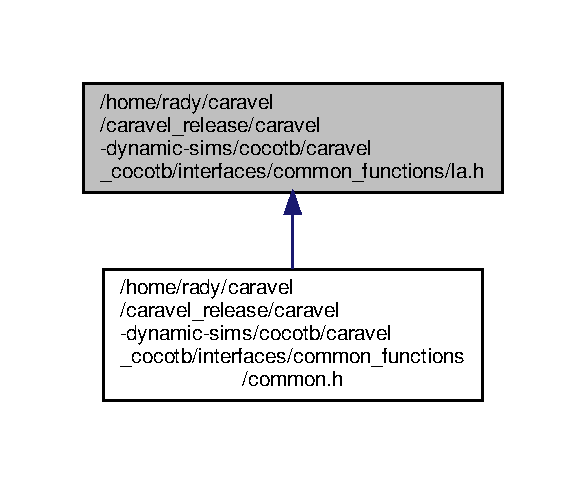
\includegraphics[width=281pt]{la_8h__dep__incl}
\end{center}
\end{figure}
\subsection*{Enumerations}
\begin{DoxyCompactItemize}
\item 
enum \hyperlink{la_8h_a4f5936f125c6714bbd6b3747270f48f0}{la\+\_\+reg\+\_\+number} 
\end{DoxyCompactItemize}
\subsection*{Functions}
\begin{DoxyCompactItemize}
\item 
void \hyperlink{la_8h_a1a3a34186b36a6386682ef6357c02746}{Logic\+Analyzer\+\_\+input\+Enable} (enum \hyperlink{la_8h_a4f5936f125c6714bbd6b3747270f48f0}{la\+\_\+reg\+\_\+number} reg\+\_\+num, unsigned int is\+\_\+enable)
\item 
void \hyperlink{la_8h_a6744740a1ac2e2d94c0057617f208de2}{Logic\+Analyzer\+\_\+output\+Enable} (enum \hyperlink{la_8h_a4f5936f125c6714bbd6b3747270f48f0}{la\+\_\+reg\+\_\+number} reg\+\_\+num, unsigned int is\+\_\+enable)
\item 
void \hyperlink{la_8h_a77a9c3c3deef468e7c5f35c5065317c5}{Logic\+Analyzer\+\_\+write} (enum \hyperlink{la_8h_a4f5936f125c6714bbd6b3747270f48f0}{la\+\_\+reg\+\_\+number} reg\+\_\+num, unsigned int data)
\item 
unsigned int \hyperlink{la_8h_acdb3e73f83b667d9ec81f0e409ad47c8}{Logic\+Analyzer\+\_\+read} (enum \hyperlink{la_8h_a4f5936f125c6714bbd6b3747270f48f0}{la\+\_\+reg\+\_\+number} reg\+\_\+num)
\end{DoxyCompactItemize}


\subsection{Enumeration Type Documentation}
\mbox{\Hypertarget{la_8h_a4f5936f125c6714bbd6b3747270f48f0}\label{la_8h_a4f5936f125c6714bbd6b3747270f48f0}} 
\index{la.\+h@{la.\+h}!la\+\_\+reg\+\_\+number@{la\+\_\+reg\+\_\+number}}
\index{la\+\_\+reg\+\_\+number@{la\+\_\+reg\+\_\+number}!la.\+h@{la.\+h}}
\subsubsection{\texorpdfstring{la\+\_\+reg\+\_\+number}{la\_reg\_number}}
{\footnotesize\ttfamily enum \hyperlink{la_8h_a4f5936f125c6714bbd6b3747270f48f0}{la\+\_\+reg\+\_\+number}}

Logic analyzers registers \hypertarget{user__space_8h_multi_row}{}
\tabulinesep=1mm
\begin{longtabu} spread 0pt [c]{*{3}{|X[-1]}|}
\caption{Enumerator la\+\_\+reg\+\_\+number}\label{user__space_8h_multi_row}\\
\hline
\rowcolor{\tableheadbgcolor}\textbf{ name}&\textbf{ value}&\textbf{ description }\\\cline{1-3}
\endfirsthead
\hline
\endfoot
\hline
\rowcolor{\tableheadbgcolor}\textbf{ name}&\textbf{ value}&\textbf{ description }\\\cline{1-3}
\endhead
L\+A\+\_\+\+R\+E\+G\+\_\+0&0&First LA register probs \mbox{[}31\+:0\mbox{]} \\\cline{1-3}
L\+A\+\_\+\+R\+E\+G\+\_\+1&1&Second LA register probs \mbox{[}63\+:32\mbox{]} \\\cline{1-3}
L\+A\+\_\+\+R\+E\+G\+\_\+2&2&Third LA register probs \mbox{[}95\+:64\mbox{]} \\\cline{1-3}
L\+A\+\_\+\+R\+E\+G\+\_\+3&3&Fourth LA register probs \mbox{[}127\+:96\mbox{]} \\\cline{1-3}
\end{longtabu}


\subsection{Function Documentation}
\mbox{\Hypertarget{la_8h_a1a3a34186b36a6386682ef6357c02746}\label{la_8h_a1a3a34186b36a6386682ef6357c02746}} 
\index{la.\+h@{la.\+h}!Logic\+Analyzer\+\_\+input\+Enable@{Logic\+Analyzer\+\_\+input\+Enable}}
\index{Logic\+Analyzer\+\_\+input\+Enable@{Logic\+Analyzer\+\_\+input\+Enable}!la.\+h@{la.\+h}}
\subsubsection{\texorpdfstring{Logic\+Analyzer\+\_\+input\+Enable()}{LogicAnalyzer\_inputEnable()}}
{\footnotesize\ttfamily void Logic\+Analyzer\+\_\+input\+Enable (\begin{DoxyParamCaption}\item[{enum \hyperlink{la_8h_a4f5936f125c6714bbd6b3747270f48f0}{la\+\_\+reg\+\_\+number}}]{reg\+\_\+num,  }\item[{unsigned int}]{is\+\_\+enable }\end{DoxyParamCaption})}

Setting logic analyzer input enable

Enable as input to the user project. firmware sends to user project


\begin{DoxyParams}{Parameters}
{\em reg\+\_\+num} & logic analyzer register to write to. Usually not all caravel versions has the same numbers of LA registers They might have 4 registers (128 probs between firmware and user project) or registers (64 probs between firmware and user project)\\
\hline
{\em is\+\_\+enable} & 32 bits each bit indicate if the corresponding probe enabled as input \\
\hline
\end{DoxyParams}
\mbox{\Hypertarget{la_8h_a6744740a1ac2e2d94c0057617f208de2}\label{la_8h_a6744740a1ac2e2d94c0057617f208de2}} 
\index{la.\+h@{la.\+h}!Logic\+Analyzer\+\_\+output\+Enable@{Logic\+Analyzer\+\_\+output\+Enable}}
\index{Logic\+Analyzer\+\_\+output\+Enable@{Logic\+Analyzer\+\_\+output\+Enable}!la.\+h@{la.\+h}}
\subsubsection{\texorpdfstring{Logic\+Analyzer\+\_\+output\+Enable()}{LogicAnalyzer\_outputEnable()}}
{\footnotesize\ttfamily void Logic\+Analyzer\+\_\+output\+Enable (\begin{DoxyParamCaption}\item[{enum \hyperlink{la_8h_a4f5936f125c6714bbd6b3747270f48f0}{la\+\_\+reg\+\_\+number}}]{reg\+\_\+num,  }\item[{unsigned int}]{is\+\_\+enable }\end{DoxyParamCaption})}

Setting logic analyzer output enable

Enable as output from the user project. firmware receives from user project


\begin{DoxyParams}{Parameters}
{\em reg\+\_\+num} & logic analyzer register to write to. Usually not all caravel versions has the same numbers of LA registers They might have 4 registers (128 probs between firmware and user project) or registers (64 probs between firmware and user project)\\
\hline
{\em is\+\_\+enable} & 32 bits each bit indicate if the corresponding probe enabled as output \\
\hline
\end{DoxyParams}
\mbox{\Hypertarget{la_8h_acdb3e73f83b667d9ec81f0e409ad47c8}\label{la_8h_acdb3e73f83b667d9ec81f0e409ad47c8}} 
\index{la.\+h@{la.\+h}!Logic\+Analyzer\+\_\+read@{Logic\+Analyzer\+\_\+read}}
\index{Logic\+Analyzer\+\_\+read@{Logic\+Analyzer\+\_\+read}!la.\+h@{la.\+h}}
\subsubsection{\texorpdfstring{Logic\+Analyzer\+\_\+read()}{LogicAnalyzer\_read()}}
{\footnotesize\ttfamily unsigned int Logic\+Analyzer\+\_\+read (\begin{DoxyParamCaption}\item[{enum \hyperlink{la_8h_a4f5936f125c6714bbd6b3747270f48f0}{la\+\_\+reg\+\_\+number}}]{reg\+\_\+num }\end{DoxyParamCaption})}

Read data through logic analyzers from user project to firmware

\begin{DoxyNote}{Note}
For this to work correctly probe should be configured as output
\end{DoxyNote}

\begin{DoxyParams}{Parameters}
{\em reg\+\_\+num} & logic analyzer register to read from. Usually not all caravel versions has the same numbers of LA registers They might have 4 registers (128 probs between firmware and user project) or registers (64 probs between firmware and user project) \\
\hline
\end{DoxyParams}
\mbox{\Hypertarget{la_8h_a77a9c3c3deef468e7c5f35c5065317c5}\label{la_8h_a77a9c3c3deef468e7c5f35c5065317c5}} 
\index{la.\+h@{la.\+h}!Logic\+Analyzer\+\_\+write@{Logic\+Analyzer\+\_\+write}}
\index{Logic\+Analyzer\+\_\+write@{Logic\+Analyzer\+\_\+write}!la.\+h@{la.\+h}}
\subsubsection{\texorpdfstring{Logic\+Analyzer\+\_\+write()}{LogicAnalyzer\_write()}}
{\footnotesize\ttfamily void Logic\+Analyzer\+\_\+write (\begin{DoxyParamCaption}\item[{enum \hyperlink{la_8h_a4f5936f125c6714bbd6b3747270f48f0}{la\+\_\+reg\+\_\+number}}]{reg\+\_\+num,  }\item[{unsigned int}]{data }\end{DoxyParamCaption})}

Write data through logic analyzers from firmware to user project

\begin{DoxyNote}{Note}
For this to work correctly probe should be configured as output
\end{DoxyNote}

\begin{DoxyParams}{Parameters}
{\em reg\+\_\+num} & logic analyzer register to write to. Usually not all caravel versions has the same numbers of LA registers They might have 4 registers (128 probs between firmware and user project) or registers (64 probs between firmware and user project)\\
\hline
{\em data} & data to write through logic analyzers \\
\hline
\end{DoxyParams}

\hypertarget{mgmt__gpio_8h}{}\section{/home/rady/caravel/caravel\+\_\+release/caravel-\/dynamic-\/sims/cocotb/caravel\+\_\+cocotb/interfaces/common\+\_\+functions/mgmt\+\_\+gpio.h File Reference}
\label{mgmt__gpio_8h}\index{/home/rady/caravel/caravel\+\_\+release/caravel-\/dynamic-\/sims/cocotb/caravel\+\_\+cocotb/interfaces/common\+\_\+functions/mgmt\+\_\+gpio.\+h@{/home/rady/caravel/caravel\+\_\+release/caravel-\/dynamic-\/sims/cocotb/caravel\+\_\+cocotb/interfaces/common\+\_\+functions/mgmt\+\_\+gpio.\+h}}
This graph shows which files directly or indirectly include this file\+:\nopagebreak
\begin{figure}[H]
\begin{center}
\leavevmode
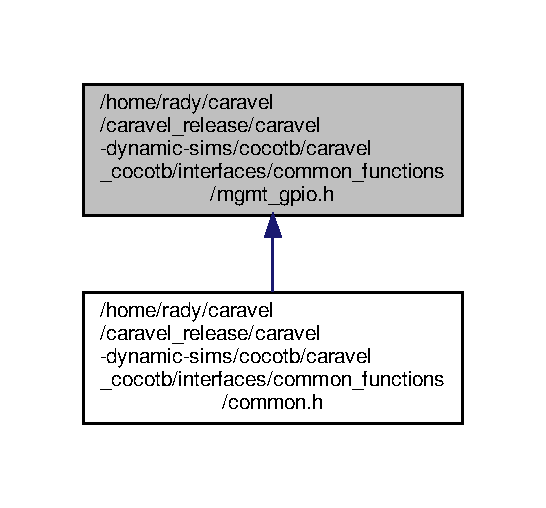
\includegraphics[width=262pt]{mgmt__gpio_8h__dep__incl}
\end{center}
\end{figure}
\subsection*{Functions}
\begin{DoxyCompactItemize}
\item 
void \hyperlink{mgmt__gpio_8h_aebb9ca3b8c8add0a6fdc5d1645a58852}{Managment\+Gpio\+\_\+input\+Enable} ()
\item 
void \hyperlink{mgmt__gpio_8h_a8e72568036b795c978c158b5c0bbd910}{Managment\+Gpio\+\_\+output\+Enable} ()
\item 
void \hyperlink{mgmt__gpio_8h_ad8433f94009bba5dfa1472264ab3f405}{Managment\+Gpio\+\_\+io\+Enable} ()
\item 
void \hyperlink{mgmt__gpio_8h_ab0d97f495e70deeb0261a968f4d83766}{Managment\+Gpio\+\_\+disable} ()
\item 
void \hyperlink{mgmt__gpio_8h_a76f7edf361e9b50ac1f91b3a2efb6d83}{Managment\+Gpio\+\_\+write} (bool data)
\item 
int \hyperlink{mgmt__gpio_8h_a1deb38550709ec95b75b81351aa97f6c}{Managment\+Gpio\+\_\+read} ()
\item 
void \hyperlink{mgmt__gpio_8h_a7f368859e2df2c12ca3c5000f8a19132}{Managment\+Gpio\+\_\+wait} (bool data)
\end{DoxyCompactItemize}


\subsection{Function Documentation}
\mbox{\Hypertarget{mgmt__gpio_8h_ab0d97f495e70deeb0261a968f4d83766}\label{mgmt__gpio_8h_ab0d97f495e70deeb0261a968f4d83766}} 
\index{mgmt\+\_\+gpio.\+h@{mgmt\+\_\+gpio.\+h}!Managment\+Gpio\+\_\+disable@{Managment\+Gpio\+\_\+disable}}
\index{Managment\+Gpio\+\_\+disable@{Managment\+Gpio\+\_\+disable}!mgmt\+\_\+gpio.\+h@{mgmt\+\_\+gpio.\+h}}
\subsubsection{\texorpdfstring{Managment\+Gpio\+\_\+disable()}{ManagmentGpio\_disable()}}
{\footnotesize\ttfamily void Managment\+Gpio\+\_\+disable (\begin{DoxyParamCaption}{ }\end{DoxyParamCaption})}

Configure management G\+P\+IO as floating It\textquotesingle{}s not connected as input or output \mbox{\Hypertarget{mgmt__gpio_8h_aebb9ca3b8c8add0a6fdc5d1645a58852}\label{mgmt__gpio_8h_aebb9ca3b8c8add0a6fdc5d1645a58852}} 
\index{mgmt\+\_\+gpio.\+h@{mgmt\+\_\+gpio.\+h}!Managment\+Gpio\+\_\+input\+Enable@{Managment\+Gpio\+\_\+input\+Enable}}
\index{Managment\+Gpio\+\_\+input\+Enable@{Managment\+Gpio\+\_\+input\+Enable}!mgmt\+\_\+gpio.\+h@{mgmt\+\_\+gpio.\+h}}
\subsubsection{\texorpdfstring{Managment\+Gpio\+\_\+input\+Enable()}{ManagmentGpio\_inputEnable()}}
{\footnotesize\ttfamily void Managment\+Gpio\+\_\+input\+Enable (\begin{DoxyParamCaption}{ }\end{DoxyParamCaption})}

Configure management G\+P\+IO as input \mbox{\Hypertarget{mgmt__gpio_8h_ad8433f94009bba5dfa1472264ab3f405}\label{mgmt__gpio_8h_ad8433f94009bba5dfa1472264ab3f405}} 
\index{mgmt\+\_\+gpio.\+h@{mgmt\+\_\+gpio.\+h}!Managment\+Gpio\+\_\+io\+Enable@{Managment\+Gpio\+\_\+io\+Enable}}
\index{Managment\+Gpio\+\_\+io\+Enable@{Managment\+Gpio\+\_\+io\+Enable}!mgmt\+\_\+gpio.\+h@{mgmt\+\_\+gpio.\+h}}
\subsubsection{\texorpdfstring{Managment\+Gpio\+\_\+io\+Enable()}{ManagmentGpio\_ioEnable()}}
{\footnotesize\ttfamily void Managment\+Gpio\+\_\+io\+Enable (\begin{DoxyParamCaption}{ }\end{DoxyParamCaption})}

Configure management G\+P\+IO as bi-\/direction \mbox{\Hypertarget{mgmt__gpio_8h_a8e72568036b795c978c158b5c0bbd910}\label{mgmt__gpio_8h_a8e72568036b795c978c158b5c0bbd910}} 
\index{mgmt\+\_\+gpio.\+h@{mgmt\+\_\+gpio.\+h}!Managment\+Gpio\+\_\+output\+Enable@{Managment\+Gpio\+\_\+output\+Enable}}
\index{Managment\+Gpio\+\_\+output\+Enable@{Managment\+Gpio\+\_\+output\+Enable}!mgmt\+\_\+gpio.\+h@{mgmt\+\_\+gpio.\+h}}
\subsubsection{\texorpdfstring{Managment\+Gpio\+\_\+output\+Enable()}{ManagmentGpio\_outputEnable()}}
{\footnotesize\ttfamily void Managment\+Gpio\+\_\+output\+Enable (\begin{DoxyParamCaption}{ }\end{DoxyParamCaption})}

Configure management G\+P\+IO as output \mbox{\Hypertarget{mgmt__gpio_8h_a1deb38550709ec95b75b81351aa97f6c}\label{mgmt__gpio_8h_a1deb38550709ec95b75b81351aa97f6c}} 
\index{mgmt\+\_\+gpio.\+h@{mgmt\+\_\+gpio.\+h}!Managment\+Gpio\+\_\+read@{Managment\+Gpio\+\_\+read}}
\index{Managment\+Gpio\+\_\+read@{Managment\+Gpio\+\_\+read}!mgmt\+\_\+gpio.\+h@{mgmt\+\_\+gpio.\+h}}
\subsubsection{\texorpdfstring{Managment\+Gpio\+\_\+read()}{ManagmentGpio\_read()}}
{\footnotesize\ttfamily int Managment\+Gpio\+\_\+read (\begin{DoxyParamCaption}{ }\end{DoxyParamCaption})}

Read data in management G\+P\+IO

\begin{DoxyNote}{Note}
This function works correctly when management G\+P\+IO configured as input If management doesn\textquotesingle{}t connect to anything the firmware would read \char`\"{}0\char`\"{} 
\end{DoxyNote}
\mbox{\Hypertarget{mgmt__gpio_8h_a7f368859e2df2c12ca3c5000f8a19132}\label{mgmt__gpio_8h_a7f368859e2df2c12ca3c5000f8a19132}} 
\index{mgmt\+\_\+gpio.\+h@{mgmt\+\_\+gpio.\+h}!Managment\+Gpio\+\_\+wait@{Managment\+Gpio\+\_\+wait}}
\index{Managment\+Gpio\+\_\+wait@{Managment\+Gpio\+\_\+wait}!mgmt\+\_\+gpio.\+h@{mgmt\+\_\+gpio.\+h}}
\subsubsection{\texorpdfstring{Managment\+Gpio\+\_\+wait()}{ManagmentGpio\_wait()}}
{\footnotesize\ttfamily void Managment\+Gpio\+\_\+wait (\begin{DoxyParamCaption}\item[{bool}]{data }\end{DoxyParamCaption})}

Wait over management G\+P\+IO to equal data

\begin{DoxyNote}{Note}
This function works correctly when management G\+P\+IO configured as input
\end{DoxyNote}

\begin{DoxyParams}{Parameters}
{\em data} & data to wait over \\
\hline
\end{DoxyParams}
\mbox{\Hypertarget{mgmt__gpio_8h_a76f7edf361e9b50ac1f91b3a2efb6d83}\label{mgmt__gpio_8h_a76f7edf361e9b50ac1f91b3a2efb6d83}} 
\index{mgmt\+\_\+gpio.\+h@{mgmt\+\_\+gpio.\+h}!Managment\+Gpio\+\_\+write@{Managment\+Gpio\+\_\+write}}
\index{Managment\+Gpio\+\_\+write@{Managment\+Gpio\+\_\+write}!mgmt\+\_\+gpio.\+h@{mgmt\+\_\+gpio.\+h}}
\subsubsection{\texorpdfstring{Managment\+Gpio\+\_\+write()}{ManagmentGpio\_write()}}
{\footnotesize\ttfamily void Managment\+Gpio\+\_\+write (\begin{DoxyParamCaption}\item[{bool}]{data }\end{DoxyParamCaption})}

Write data in management G\+P\+IO


\begin{DoxyParams}{Parameters}
{\em data} & data to write at management G\+P\+IO possible values are 0 and 1\\
\hline
\end{DoxyParams}
\begin{DoxyNote}{Note}
This function works when management G\+P\+IO configured as output 
\end{DoxyNote}

\hypertarget{spi__master_8h}{}\section{/home/rady/caravel/caravel\+\_\+release/caravel-\/dynamic-\/sims/cocotb/caravel\+\_\+cocotb/interfaces/common\+\_\+functions/spi\+\_\+master.h File Reference}
\label{spi__master_8h}\index{/home/rady/caravel/caravel\+\_\+release/caravel-\/dynamic-\/sims/cocotb/caravel\+\_\+cocotb/interfaces/common\+\_\+functions/spi\+\_\+master.\+h@{/home/rady/caravel/caravel\+\_\+release/caravel-\/dynamic-\/sims/cocotb/caravel\+\_\+cocotb/interfaces/common\+\_\+functions/spi\+\_\+master.\+h}}
This graph shows which files directly or indirectly include this file\+:\nopagebreak
\begin{figure}[H]
\begin{center}
\leavevmode
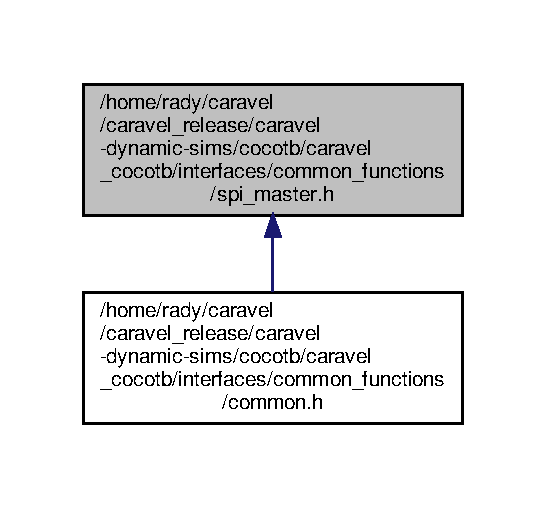
\includegraphics[width=262pt]{spi__master_8h__dep__incl}
\end{center}
\end{figure}
\subsection*{Functions}
\begin{DoxyCompactItemize}
\item 
void \hyperlink{spi__master_8h_a83bfbffc1add606c915c72d53b74b0b9}{M\+S\+P\+I\+\_\+write} (char c)
\item 
char \hyperlink{spi__master_8h_add88f1c01868dbb6f7a30ca1c1ae6cf4}{M\+S\+P\+I\+\_\+read} ()
\item 
void \hyperlink{spi__master_8h_aaa60b306dd0fc9f21f6d10b7fa08034d}{M\+S\+P\+I\+\_\+enable} (bool is\+\_\+enable)
\item 
void \hyperlink{spi__master_8h_abe298fb2168613cf2e43af17404b3aad}{M\+S\+P\+I\+\_\+enable\+CS} (bool is\+\_\+enable)
\end{DoxyCompactItemize}


\subsection{Function Documentation}
\mbox{\Hypertarget{spi__master_8h_aaa60b306dd0fc9f21f6d10b7fa08034d}\label{spi__master_8h_aaa60b306dd0fc9f21f6d10b7fa08034d}} 
\index{spi\+\_\+master.\+h@{spi\+\_\+master.\+h}!M\+S\+P\+I\+\_\+enable@{M\+S\+P\+I\+\_\+enable}}
\index{M\+S\+P\+I\+\_\+enable@{M\+S\+P\+I\+\_\+enable}!spi\+\_\+master.\+h@{spi\+\_\+master.\+h}}
\subsubsection{\texorpdfstring{M\+S\+P\+I\+\_\+enable()}{MSPI\_enable()}}
{\footnotesize\ttfamily void M\+S\+P\+I\+\_\+enable (\begin{DoxyParamCaption}\item[{bool}]{is\+\_\+enable }\end{DoxyParamCaption})}

Enable or disable the master S\+PI


\begin{DoxyParams}{Parameters}
{\em is\+\_\+enable} & when 1 (true) master S\+PI is active, 0 (false) master S\+PI is disabled \\
\hline
\end{DoxyParams}
\mbox{\Hypertarget{spi__master_8h_abe298fb2168613cf2e43af17404b3aad}\label{spi__master_8h_abe298fb2168613cf2e43af17404b3aad}} 
\index{spi\+\_\+master.\+h@{spi\+\_\+master.\+h}!M\+S\+P\+I\+\_\+enable\+CS@{M\+S\+P\+I\+\_\+enable\+CS}}
\index{M\+S\+P\+I\+\_\+enable\+CS@{M\+S\+P\+I\+\_\+enable\+CS}!spi\+\_\+master.\+h@{spi\+\_\+master.\+h}}
\subsubsection{\texorpdfstring{M\+S\+P\+I\+\_\+enable\+C\+S()}{MSPI\_enableCS()}}
{\footnotesize\ttfamily void M\+S\+P\+I\+\_\+enable\+CS (\begin{DoxyParamCaption}\item[{bool}]{is\+\_\+enable }\end{DoxyParamCaption})}

assert or deassert chip select


\begin{DoxyParams}{Parameters}
{\em is\+\_\+enable} & when 1 (true) chip select is asserted, 0 (false) chip select is deasserted \\
\hline
\end{DoxyParams}
\mbox{\Hypertarget{spi__master_8h_add88f1c01868dbb6f7a30ca1c1ae6cf4}\label{spi__master_8h_add88f1c01868dbb6f7a30ca1c1ae6cf4}} 
\index{spi\+\_\+master.\+h@{spi\+\_\+master.\+h}!M\+S\+P\+I\+\_\+read@{M\+S\+P\+I\+\_\+read}}
\index{M\+S\+P\+I\+\_\+read@{M\+S\+P\+I\+\_\+read}!spi\+\_\+master.\+h@{spi\+\_\+master.\+h}}
\subsubsection{\texorpdfstring{M\+S\+P\+I\+\_\+read()}{MSPI\_read()}}
{\footnotesize\ttfamily char M\+S\+P\+I\+\_\+read (\begin{DoxyParamCaption}{ }\end{DoxyParamCaption})}

Read byte (8bits) through S\+PI master \mbox{\Hypertarget{spi__master_8h_a83bfbffc1add606c915c72d53b74b0b9}\label{spi__master_8h_a83bfbffc1add606c915c72d53b74b0b9}} 
\index{spi\+\_\+master.\+h@{spi\+\_\+master.\+h}!M\+S\+P\+I\+\_\+write@{M\+S\+P\+I\+\_\+write}}
\index{M\+S\+P\+I\+\_\+write@{M\+S\+P\+I\+\_\+write}!spi\+\_\+master.\+h@{spi\+\_\+master.\+h}}
\subsubsection{\texorpdfstring{M\+S\+P\+I\+\_\+write()}{MSPI\_write()}}
{\footnotesize\ttfamily void M\+S\+P\+I\+\_\+write (\begin{DoxyParamCaption}\item[{char}]{c }\end{DoxyParamCaption})}

Write byte (8bits) through S\+PI master


\begin{DoxyParams}{Parameters}
{\em c} & byte to write range 0x0 to 0x\+FF \\
\hline
\end{DoxyParams}

\hypertarget{timer0_8h}{}\section{/home/rady/caravel/caravel\+\_\+release/caravel-\/dynamic-\/sims/cocotb/caravel\+\_\+cocotb/interfaces/common\+\_\+functions/timer0.h File Reference}
\label{timer0_8h}\index{/home/rady/caravel/caravel\+\_\+release/caravel-\/dynamic-\/sims/cocotb/caravel\+\_\+cocotb/interfaces/common\+\_\+functions/timer0.\+h@{/home/rady/caravel/caravel\+\_\+release/caravel-\/dynamic-\/sims/cocotb/caravel\+\_\+cocotb/interfaces/common\+\_\+functions/timer0.\+h}}
This graph shows which files directly or indirectly include this file\+:\nopagebreak
\begin{figure}[H]
\begin{center}
\leavevmode
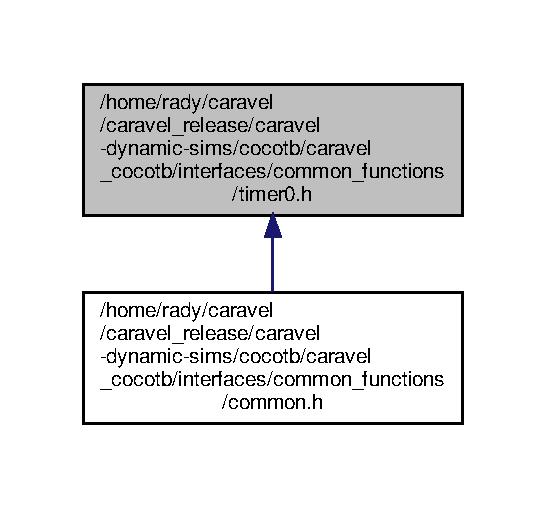
\includegraphics[width=262pt]{timer0_8h__dep__incl}
\end{center}
\end{figure}
\subsection*{Functions}
\begin{DoxyCompactItemize}
\item 
void \hyperlink{timer0_8h_a2400e05d4063a49d5e0881a8e422ec86}{timer0\+\_\+configure\+One\+Shot} (unsigned int count)
\item 
void \hyperlink{timer0_8h_a06884fc27bfe7793f6904774b6565b25}{timer0\+\_\+configure\+Periodic} (unsigned int count)
\item 
void \hyperlink{timer0_8h_a2974c941008418ea21ba4641f83c4ea7}{timer0\+\_\+enable} (bool is\+\_\+enable)
\item 
unsigned int \hyperlink{timer0_8h_ac86682420d0de4bab7bf133f67e6e35b}{timer0\+\_\+read\+Value} ()
\end{DoxyCompactItemize}


\subsection{Function Documentation}
\mbox{\Hypertarget{timer0_8h_a2400e05d4063a49d5e0881a8e422ec86}\label{timer0_8h_a2400e05d4063a49d5e0881a8e422ec86}} 
\index{timer0.\+h@{timer0.\+h}!timer0\+\_\+configure\+One\+Shot@{timer0\+\_\+configure\+One\+Shot}}
\index{timer0\+\_\+configure\+One\+Shot@{timer0\+\_\+configure\+One\+Shot}!timer0.\+h@{timer0.\+h}}
\subsubsection{\texorpdfstring{timer0\+\_\+configure\+One\+Shot()}{timer0\_configureOneShot()}}
{\footnotesize\ttfamily void timer0\+\_\+configure\+One\+Shot (\begin{DoxyParamCaption}\item[{unsigned int}]{count }\end{DoxyParamCaption})}

Start Timer in oneshot countdown mode start value is count


\begin{DoxyParams}{Parameters}
{\em count} & start value in the counter $>$ 0 \\
\hline
\end{DoxyParams}
\mbox{\Hypertarget{timer0_8h_a06884fc27bfe7793f6904774b6565b25}\label{timer0_8h_a06884fc27bfe7793f6904774b6565b25}} 
\index{timer0.\+h@{timer0.\+h}!timer0\+\_\+configure\+Periodic@{timer0\+\_\+configure\+Periodic}}
\index{timer0\+\_\+configure\+Periodic@{timer0\+\_\+configure\+Periodic}!timer0.\+h@{timer0.\+h}}
\subsubsection{\texorpdfstring{timer0\+\_\+configure\+Periodic()}{timer0\_configurePeriodic()}}
{\footnotesize\ttfamily void timer0\+\_\+configure\+Periodic (\begin{DoxyParamCaption}\item[{unsigned int}]{count }\end{DoxyParamCaption})}

Start counter in periodic countdown mode start value is count

Timer will roll over to the count value when it reaches 0 
\begin{DoxyParams}{Parameters}
{\em count} & start value in the counter $>$ 0 \\
\hline
\end{DoxyParams}
\mbox{\Hypertarget{timer0_8h_a2974c941008418ea21ba4641f83c4ea7}\label{timer0_8h_a2974c941008418ea21ba4641f83c4ea7}} 
\index{timer0.\+h@{timer0.\+h}!timer0\+\_\+enable@{timer0\+\_\+enable}}
\index{timer0\+\_\+enable@{timer0\+\_\+enable}!timer0.\+h@{timer0.\+h}}
\subsubsection{\texorpdfstring{timer0\+\_\+enable()}{timer0\_enable()}}
{\footnotesize\ttfamily void timer0\+\_\+enable (\begin{DoxyParamCaption}\item[{bool}]{is\+\_\+enable }\end{DoxyParamCaption})}

Enable or Disable timer0


\begin{DoxyParams}{Parameters}
{\em is\+\_\+enable} & when 1 (true) timer0 is enable (start counting), 0 (false) timer0 is disabled \\
\hline
\end{DoxyParams}
\mbox{\Hypertarget{timer0_8h_ac86682420d0de4bab7bf133f67e6e35b}\label{timer0_8h_ac86682420d0de4bab7bf133f67e6e35b}} 
\index{timer0.\+h@{timer0.\+h}!timer0\+\_\+read\+Value@{timer0\+\_\+read\+Value}}
\index{timer0\+\_\+read\+Value@{timer0\+\_\+read\+Value}!timer0.\+h@{timer0.\+h}}
\subsubsection{\texorpdfstring{timer0\+\_\+read\+Value()}{timer0\_readValue()}}
{\footnotesize\ttfamily unsigned int timer0\+\_\+read\+Value (\begin{DoxyParamCaption}{ }\end{DoxyParamCaption})}

Get timer current value 
\hypertarget{uart__api_8h}{}\section{/home/rady/caravel/caravel\+\_\+release/caravel-\/dynamic-\/sims/cocotb/caravel\+\_\+cocotb/interfaces/common\+\_\+functions/uart\+\_\+api.h File Reference}
\label{uart__api_8h}\index{/home/rady/caravel/caravel\+\_\+release/caravel-\/dynamic-\/sims/cocotb/caravel\+\_\+cocotb/interfaces/common\+\_\+functions/uart\+\_\+api.\+h@{/home/rady/caravel/caravel\+\_\+release/caravel-\/dynamic-\/sims/cocotb/caravel\+\_\+cocotb/interfaces/common\+\_\+functions/uart\+\_\+api.\+h}}
This graph shows which files directly or indirectly include this file\+:\nopagebreak
\begin{figure}[H]
\begin{center}
\leavevmode
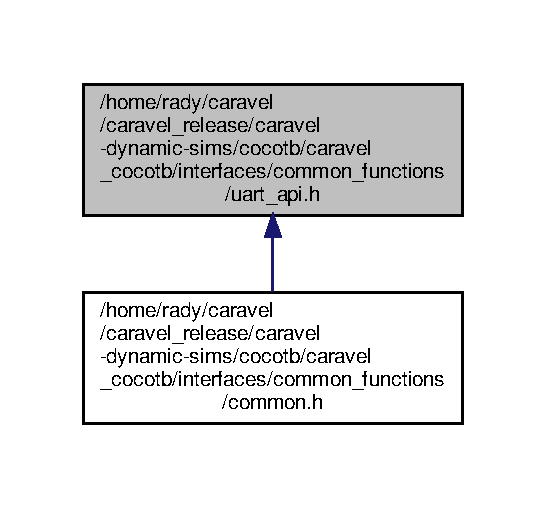
\includegraphics[width=262pt]{uart__api_8h__dep__incl}
\end{center}
\end{figure}
\subsection*{Functions}
\begin{DoxyCompactItemize}
\item 
void \hyperlink{uart__api_8h_aca637427323a13558b46e2ee65f6638b}{U\+A\+R\+T\+\_\+enable\+TX} (bool is\+\_\+enable)
\item 
void \hyperlink{uart__api_8h_ac7e8b94a1b33769e737169c6fa338912}{U\+A\+R\+T\+\_\+enable\+RX} (bool is\+\_\+enable)
\item 
char \hyperlink{uart__api_8h_a6e0d67a7b5c73e1133d8906eb2037c14}{U\+A\+R\+T\+\_\+read\+Char} ()
\item 
void \hyperlink{uart__api_8h_accbd12d45ca5357084a42e65f30c7379}{U\+A\+R\+T\+\_\+pop\+Char} ()
\item 
char $\ast$ \hyperlink{uart__api_8h_a0a812bb491942a62046e93a592ce5225}{U\+A\+R\+T\+\_\+read\+Line} ()
\item 
void \hyperlink{uart__api_8h_a2d0091e019fc1a50c3cc9f4c86dd73c2}{print} (const char $\ast$p)
\item 
void \hyperlink{uart__api_8h_a69895a7561310168b024cca863b23206}{U\+A\+R\+T\+\_\+send\+Char} (char c)
\item 
void \hyperlink{uart__api_8h_a09274b38f8919ad158c0d1ec38271059}{U\+A\+R\+T\+\_\+send\+Int} (int data)
\end{DoxyCompactItemize}


\subsection{Function Documentation}
\mbox{\Hypertarget{uart__api_8h_a2d0091e019fc1a50c3cc9f4c86dd73c2}\label{uart__api_8h_a2d0091e019fc1a50c3cc9f4c86dd73c2}} 
\index{uart\+\_\+api.\+h@{uart\+\_\+api.\+h}!print@{print}}
\index{print@{print}!uart\+\_\+api.\+h@{uart\+\_\+api.\+h}}
\subsubsection{\texorpdfstring{print()}{print()}}
{\footnotesize\ttfamily void print (\begin{DoxyParamCaption}\item[{const char $\ast$}]{p }\end{DoxyParamCaption})}

Send A\+S\+C\+II symbol or symbols through U\+A\+RT

TX mode have to be enabled \mbox{\Hypertarget{uart__api_8h_ac7e8b94a1b33769e737169c6fa338912}\label{uart__api_8h_ac7e8b94a1b33769e737169c6fa338912}} 
\index{uart\+\_\+api.\+h@{uart\+\_\+api.\+h}!U\+A\+R\+T\+\_\+enable\+RX@{U\+A\+R\+T\+\_\+enable\+RX}}
\index{U\+A\+R\+T\+\_\+enable\+RX@{U\+A\+R\+T\+\_\+enable\+RX}!uart\+\_\+api.\+h@{uart\+\_\+api.\+h}}
\subsubsection{\texorpdfstring{U\+A\+R\+T\+\_\+enable\+R\+X()}{UART\_enableRX()}}
{\footnotesize\ttfamily void U\+A\+R\+T\+\_\+enable\+RX (\begin{DoxyParamCaption}\item[{bool}]{is\+\_\+enable }\end{DoxyParamCaption})}

Enable or disable RX of U\+A\+RT


\begin{DoxyParams}{Parameters}
{\em is\+\_\+enable} & when 1(true) U\+A\+RT RX enable, 0 (false) U\+A\+RT RX disable\\
\hline
\end{DoxyParams}
\begin{DoxyNote}{Note}
Some caravel C\+PU enable and disable U\+A\+RT TX and RX together 
\end{DoxyNote}
\mbox{\Hypertarget{uart__api_8h_aca637427323a13558b46e2ee65f6638b}\label{uart__api_8h_aca637427323a13558b46e2ee65f6638b}} 
\index{uart\+\_\+api.\+h@{uart\+\_\+api.\+h}!U\+A\+R\+T\+\_\+enable\+TX@{U\+A\+R\+T\+\_\+enable\+TX}}
\index{U\+A\+R\+T\+\_\+enable\+TX@{U\+A\+R\+T\+\_\+enable\+TX}!uart\+\_\+api.\+h@{uart\+\_\+api.\+h}}
\subsubsection{\texorpdfstring{U\+A\+R\+T\+\_\+enable\+T\+X()}{UART\_enableTX()}}
{\footnotesize\ttfamily void U\+A\+R\+T\+\_\+enable\+TX (\begin{DoxyParamCaption}\item[{bool}]{is\+\_\+enable }\end{DoxyParamCaption})}

Enable or disable TX of U\+A\+RT


\begin{DoxyParams}{Parameters}
{\em is\+\_\+enable} & when 1(true) U\+A\+RT TX enable, 0 (false) U\+A\+RT TX disable\\
\hline
\end{DoxyParams}
\begin{DoxyNote}{Note}
Some caravel C\+PU enable and disable U\+A\+RT TX and RX together 
\end{DoxyNote}
\mbox{\Hypertarget{uart__api_8h_accbd12d45ca5357084a42e65f30c7379}\label{uart__api_8h_accbd12d45ca5357084a42e65f30c7379}} 
\index{uart\+\_\+api.\+h@{uart\+\_\+api.\+h}!U\+A\+R\+T\+\_\+pop\+Char@{U\+A\+R\+T\+\_\+pop\+Char}}
\index{U\+A\+R\+T\+\_\+pop\+Char@{U\+A\+R\+T\+\_\+pop\+Char}!uart\+\_\+api.\+h@{uart\+\_\+api.\+h}}
\subsubsection{\texorpdfstring{U\+A\+R\+T\+\_\+pop\+Char()}{UART\_popChar()}}
{\footnotesize\ttfamily void U\+A\+R\+T\+\_\+pop\+Char (\begin{DoxyParamCaption}{ }\end{DoxyParamCaption})}

Pop the first A\+S\+C\+II symbol of the U\+A\+RT received queue

\hyperlink{uart__api_8h_a6e0d67a7b5c73e1133d8906eb2037c14}{U\+A\+R\+T\+\_\+read\+Char()} function would keeping reading the same symbol unless this function is called \mbox{\Hypertarget{uart__api_8h_a6e0d67a7b5c73e1133d8906eb2037c14}\label{uart__api_8h_a6e0d67a7b5c73e1133d8906eb2037c14}} 
\index{uart\+\_\+api.\+h@{uart\+\_\+api.\+h}!U\+A\+R\+T\+\_\+read\+Char@{U\+A\+R\+T\+\_\+read\+Char}}
\index{U\+A\+R\+T\+\_\+read\+Char@{U\+A\+R\+T\+\_\+read\+Char}!uart\+\_\+api.\+h@{uart\+\_\+api.\+h}}
\subsubsection{\texorpdfstring{U\+A\+R\+T\+\_\+read\+Char()}{UART\_readChar()}}
{\footnotesize\ttfamily char U\+A\+R\+T\+\_\+read\+Char (\begin{DoxyParamCaption}{ }\end{DoxyParamCaption})}

Wait receiving A\+S\+C\+II symbol and return it.

Return the first A\+S\+C\+II symbol of the U\+A\+RT received queue

RX mode have to be enabled \mbox{\Hypertarget{uart__api_8h_a0a812bb491942a62046e93a592ce5225}\label{uart__api_8h_a0a812bb491942a62046e93a592ce5225}} 
\index{uart\+\_\+api.\+h@{uart\+\_\+api.\+h}!U\+A\+R\+T\+\_\+read\+Line@{U\+A\+R\+T\+\_\+read\+Line}}
\index{U\+A\+R\+T\+\_\+read\+Line@{U\+A\+R\+T\+\_\+read\+Line}!uart\+\_\+api.\+h@{uart\+\_\+api.\+h}}
\subsubsection{\texorpdfstring{U\+A\+R\+T\+\_\+read\+Line()}{UART\_readLine()}}
{\footnotesize\ttfamily char$\ast$ U\+A\+R\+T\+\_\+read\+Line (\begin{DoxyParamCaption}{ }\end{DoxyParamCaption})}

read full line msg and return it \mbox{\Hypertarget{uart__api_8h_a69895a7561310168b024cca863b23206}\label{uart__api_8h_a69895a7561310168b024cca863b23206}} 
\index{uart\+\_\+api.\+h@{uart\+\_\+api.\+h}!U\+A\+R\+T\+\_\+send\+Char@{U\+A\+R\+T\+\_\+send\+Char}}
\index{U\+A\+R\+T\+\_\+send\+Char@{U\+A\+R\+T\+\_\+send\+Char}!uart\+\_\+api.\+h@{uart\+\_\+api.\+h}}
\subsubsection{\texorpdfstring{U\+A\+R\+T\+\_\+send\+Char()}{UART\_sendChar()}}
{\footnotesize\ttfamily void U\+A\+R\+T\+\_\+send\+Char (\begin{DoxyParamCaption}\item[{char}]{c }\end{DoxyParamCaption})}

Send A\+S\+C\+II char through U\+A\+RT 
\begin{DoxyParams}{Parameters}
{\em c} & A\+S\+C\+II char to send\\
\hline
\end{DoxyParams}
TX mode have to be enabled \mbox{\Hypertarget{uart__api_8h_a09274b38f8919ad158c0d1ec38271059}\label{uart__api_8h_a09274b38f8919ad158c0d1ec38271059}} 
\index{uart\+\_\+api.\+h@{uart\+\_\+api.\+h}!U\+A\+R\+T\+\_\+send\+Int@{U\+A\+R\+T\+\_\+send\+Int}}
\index{U\+A\+R\+T\+\_\+send\+Int@{U\+A\+R\+T\+\_\+send\+Int}!uart\+\_\+api.\+h@{uart\+\_\+api.\+h}}
\subsubsection{\texorpdfstring{U\+A\+R\+T\+\_\+send\+Int()}{UART\_sendInt()}}
{\footnotesize\ttfamily void U\+A\+R\+T\+\_\+send\+Int (\begin{DoxyParamCaption}\item[{int}]{data }\end{DoxyParamCaption})}

Send int through U\+A\+RT the int would be sent as 8 hex characters 
\begin{DoxyParams}{Parameters}
{\em c} & int to send\\
\hline
\end{DoxyParams}
TX mode have to be enabled 
\hypertarget{user__space_8h}{}\section{/home/rady/caravel/caravel\+\_\+release/caravel-\/dynamic-\/sims/cocotb/caravel\+\_\+cocotb/interfaces/common\+\_\+functions/user\+\_\+space.h File Reference}
\label{user__space_8h}\index{/home/rady/caravel/caravel\+\_\+release/caravel-\/dynamic-\/sims/cocotb/caravel\+\_\+cocotb/interfaces/common\+\_\+functions/user\+\_\+space.\+h@{/home/rady/caravel/caravel\+\_\+release/caravel-\/dynamic-\/sims/cocotb/caravel\+\_\+cocotb/interfaces/common\+\_\+functions/user\+\_\+space.\+h}}
This graph shows which files directly or indirectly include this file\+:\nopagebreak
\begin{figure}[H]
\begin{center}
\leavevmode
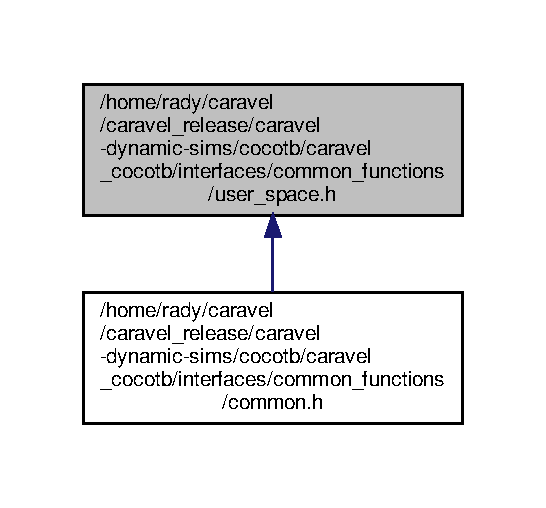
\includegraphics[width=262pt]{user__space_8h__dep__incl}
\end{center}
\end{figure}
\subsection*{Functions}
\begin{DoxyCompactItemize}
\item 
void \hyperlink{user__space_8h_a613cc002383517796ba21968f75c0ff4}{User\+\_\+enable\+IF} ()
\item 
void \hyperlink{user__space_8h_ab4b69057d303df38c571ff19fe70d760}{U\+S\+E\+R\+\_\+write\+Word} (unsigned int data, int offset)
\item 
unsigned int \hyperlink{user__space_8h_a8341444d1c6a9834627a08284b86bdfd}{U\+S\+E\+R\+\_\+read\+Word} (int offset)
\item 
void \hyperlink{user__space_8h_a3aa2a0b36d2fea89e3540866fa878505}{U\+S\+E\+R\+\_\+write\+Half\+Word} (unsigned short data, unsigned int offset, bool is\+\_\+first\+\_\+word)
\item 
unsigned short \hyperlink{user__space_8h_ad5f4e621258f311f860ee139078d402b}{U\+S\+E\+R\+\_\+read\+Half\+Word} (unsigned int offset, bool is\+\_\+first\+\_\+word)
\item 
void \hyperlink{user__space_8h_a9cda3d41541035be2198550b85cd1a5f}{U\+S\+E\+R\+\_\+write\+Byte} (unsigned char data, unsigned int offset, unsigned char byte\+\_\+num)
\item 
unsigned char \hyperlink{user__space_8h_a4d1bd64c76584c644c5c30091b6a2380}{U\+S\+E\+R\+\_\+read\+Byte} (unsigned int offset, unsigned char byte\+\_\+num)
\end{DoxyCompactItemize}


\subsection{Function Documentation}
\mbox{\Hypertarget{user__space_8h_a613cc002383517796ba21968f75c0ff4}\label{user__space_8h_a613cc002383517796ba21968f75c0ff4}} 
\index{user\+\_\+space.\+h@{user\+\_\+space.\+h}!User\+\_\+enable\+IF@{User\+\_\+enable\+IF}}
\index{User\+\_\+enable\+IF@{User\+\_\+enable\+IF}!user\+\_\+space.\+h@{user\+\_\+space.\+h}}
\subsubsection{\texorpdfstring{User\+\_\+enable\+I\+F()}{User\_enableIF()}}
{\footnotesize\ttfamily void User\+\_\+enable\+IF (\begin{DoxyParamCaption}{ }\end{DoxyParamCaption})}

Enable communication between firmware and user project through wishbone \begin{DoxyWarning}{Warning}
This necessary when reading or writing are needed between wishbone and user project if interface isn\textquotesingle{}t enabled no ack would be receive and the writing or reading command will be stuck 
\end{DoxyWarning}
\mbox{\Hypertarget{user__space_8h_a4d1bd64c76584c644c5c30091b6a2380}\label{user__space_8h_a4d1bd64c76584c644c5c30091b6a2380}} 
\index{user\+\_\+space.\+h@{user\+\_\+space.\+h}!U\+S\+E\+R\+\_\+read\+Byte@{U\+S\+E\+R\+\_\+read\+Byte}}
\index{U\+S\+E\+R\+\_\+read\+Byte@{U\+S\+E\+R\+\_\+read\+Byte}!user\+\_\+space.\+h@{user\+\_\+space.\+h}}
\subsubsection{\texorpdfstring{U\+S\+E\+R\+\_\+read\+Byte()}{USER\_readByte()}}
{\footnotesize\ttfamily unsigned char U\+S\+E\+R\+\_\+read\+Byte (\begin{DoxyParamCaption}\item[{unsigned int}]{offset,  }\item[{unsigned char}]{byte\+\_\+num }\end{DoxyParamCaption})}

Read byte at user address space 32 bit register


\begin{DoxyParams}{Parameters}
{\em offset} & the offset of the register to write. Origin at the user project address \\
\hline
{\em byte\+\_\+num} & number of the in the 4 bytes register (32 bits)\\
\hline
\end{DoxyParams}
\begin{DoxyNote}{Note}
Since offset is a word (4 bytes) and address space represent bytes, offset = address /4 ~\newline
 For example if project caravel space are 26 address bit offset = wb\+\_\+addr\+\_\+i\mbox{[}25\+:0\mbox{]}/4
\end{DoxyNote}
\hypertarget{user__space_8h_multi_row}{}
\tabulinesep=1mm
\begin{longtabu} spread 0pt [c]{*{6}{|X[-1]}|}
\caption{world memory (2byte offset)}\label{user__space_8h_multi_row}\\
\hline
\rowcolor{\tableheadbgcolor}\textbf{ byte\+\_\+num}&\textbf{ -\/}&\textbf{ 0 }&\textbf{ 1}&\textbf{ 2}&\textbf{ 3 }\\\cline{1-6}
\endfirsthead
\hline
\endfoot
\hline
\rowcolor{\tableheadbgcolor}\textbf{ byte\+\_\+num}&\textbf{ -\/}&\textbf{ 0 }&\textbf{ 1}&\textbf{ 2}&\textbf{ 3 }\\\cline{1-6}
\endhead
\rowcolor{\tableheadbgcolor}\textbf{ address}&\textbf{ offset }&\textbf{ byte0}&\textbf{ byte1}&\textbf{ byte2}&\textbf{ byte3 }\\\cline{1-6}
0x0&0&0&1&2&3 \\\cline{1-6}
0x4&1&4&5&6&7 \\\cline{1-6}
0x8&2&8&9&10&11 \\\cline{1-6}
0xC&3&12&13&14&15 \\\cline{1-6}
\end{longtabu}
\mbox{\Hypertarget{user__space_8h_ad5f4e621258f311f860ee139078d402b}\label{user__space_8h_ad5f4e621258f311f860ee139078d402b}} 
\index{user\+\_\+space.\+h@{user\+\_\+space.\+h}!U\+S\+E\+R\+\_\+read\+Half\+Word@{U\+S\+E\+R\+\_\+read\+Half\+Word}}
\index{U\+S\+E\+R\+\_\+read\+Half\+Word@{U\+S\+E\+R\+\_\+read\+Half\+Word}!user\+\_\+space.\+h@{user\+\_\+space.\+h}}
\subsubsection{\texorpdfstring{U\+S\+E\+R\+\_\+read\+Half\+Word()}{USER\_readHalfWord()}}
{\footnotesize\ttfamily unsigned short U\+S\+E\+R\+\_\+read\+Half\+Word (\begin{DoxyParamCaption}\item[{unsigned int}]{offset,  }\item[{bool}]{is\+\_\+first\+\_\+word }\end{DoxyParamCaption})}

Read half word (2 bytes) at user address space 32 bit register


\begin{DoxyParams}{Parameters}
{\em offset} & the offset of the register to write. Origin at the user project address \\
\hline
{\em is\+\_\+first\+\_\+word} & the offset of the register to write. Origin at the user project address\\
\hline
\end{DoxyParams}
\begin{DoxyNote}{Note}
Since offset is a word (4 bytes) and address space represent bytes, offset = address /4 ~\newline
 For example if project caravel space are 26 address bit offset = wb\+\_\+addr\+\_\+i\mbox{[}25\+:0\mbox{]}/4
\end{DoxyNote}
\hypertarget{user__space_8h_multi_row}{}
\tabulinesep=1mm
\begin{longtabu} spread 0pt [c]{*{6}{|X[-1]}|}
\caption{world memory (2byte offset)}\label{user__space_8h_multi_row}\\
\hline
\rowcolor{\tableheadbgcolor}\textbf{ is first word}&\textbf{ -\/}&\textbf{ 1}&\textbf{ 1 }&\textbf{ 0}&\textbf{ 0 }\\\cline{1-6}
\endfirsthead
\hline
\endfoot
\hline
\rowcolor{\tableheadbgcolor}\textbf{ is first word}&\textbf{ -\/}&\textbf{ 1}&\textbf{ 1 }&\textbf{ 0}&\textbf{ 0 }\\\cline{1-6}
\endhead
\rowcolor{\tableheadbgcolor}\textbf{ address}&\textbf{ offset }&\textbf{ byte0}&\textbf{ byte1}&\textbf{ byte2}&\textbf{ byte3 }\\\cline{1-6}
0x0&0&0&1&2&3 \\\cline{1-6}
0x4&1&4&5&6&7 \\\cline{1-6}
0x8&2&8&9&10&11 \\\cline{1-6}
0xC&3&12&13&14&15 \\\cline{1-6}
\end{longtabu}
\mbox{\Hypertarget{user__space_8h_a8341444d1c6a9834627a08284b86bdfd}\label{user__space_8h_a8341444d1c6a9834627a08284b86bdfd}} 
\index{user\+\_\+space.\+h@{user\+\_\+space.\+h}!U\+S\+E\+R\+\_\+read\+Word@{U\+S\+E\+R\+\_\+read\+Word}}
\index{U\+S\+E\+R\+\_\+read\+Word@{U\+S\+E\+R\+\_\+read\+Word}!user\+\_\+space.\+h@{user\+\_\+space.\+h}}
\subsubsection{\texorpdfstring{U\+S\+E\+R\+\_\+read\+Word()}{USER\_readWord()}}
{\footnotesize\ttfamily unsigned int U\+S\+E\+R\+\_\+read\+Word (\begin{DoxyParamCaption}\item[{int}]{offset }\end{DoxyParamCaption})}

Read word (4 bytes) at user address space 32 bit register


\begin{DoxyParams}{Parameters}
{\em offset} & the offset of the register to write. Origin at the user project address\\
\hline
\end{DoxyParams}
\begin{DoxyNote}{Note}
Since offset is a word (4 bytes) and address space represent bytes, offset = address /4 ~\newline
 For example if project caravel space are 26 address bit offset = wb\+\_\+addr\+\_\+i\mbox{[}25\+:0\mbox{]}/4
\end{DoxyNote}
\hypertarget{user__space_8h_multi_row}{}
\tabulinesep=1mm
\begin{longtabu} spread 0pt [c]{*{6}{|X[-1]}|}
\caption{world memory (4 bytes offset)}\label{user__space_8h_multi_row}\\
\hline
\rowcolor{\tableheadbgcolor}\textbf{ address}&\textbf{ offset }&\textbf{ byte0}&\textbf{ byte1}&\textbf{ byte2}&\textbf{ byte3 }\\\cline{1-6}
\endfirsthead
\hline
\endfoot
\hline
\rowcolor{\tableheadbgcolor}\textbf{ address}&\textbf{ offset }&\textbf{ byte0}&\textbf{ byte1}&\textbf{ byte2}&\textbf{ byte3 }\\\cline{1-6}
\endhead
0x0&0&0&1&2&3 \\\cline{1-6}
0x4&1&4&5&6&7 \\\cline{1-6}
0x8&2&8&9&10&11 \\\cline{1-6}
0xC&3&12&13&14&15 \\\cline{1-6}
\end{longtabu}
\mbox{\Hypertarget{user__space_8h_a9cda3d41541035be2198550b85cd1a5f}\label{user__space_8h_a9cda3d41541035be2198550b85cd1a5f}} 
\index{user\+\_\+space.\+h@{user\+\_\+space.\+h}!U\+S\+E\+R\+\_\+write\+Byte@{U\+S\+E\+R\+\_\+write\+Byte}}
\index{U\+S\+E\+R\+\_\+write\+Byte@{U\+S\+E\+R\+\_\+write\+Byte}!user\+\_\+space.\+h@{user\+\_\+space.\+h}}
\subsubsection{\texorpdfstring{U\+S\+E\+R\+\_\+write\+Byte()}{USER\_writeByte()}}
{\footnotesize\ttfamily void U\+S\+E\+R\+\_\+write\+Byte (\begin{DoxyParamCaption}\item[{unsigned char}]{data,  }\item[{unsigned int}]{offset,  }\item[{unsigned char}]{byte\+\_\+num }\end{DoxyParamCaption})}

Write byte at user address space 32 bit register


\begin{DoxyParams}{Parameters}
{\em data} & byte data to write \\
\hline
{\em offset} & the offset of the register to write. Origin at the user project address \\
\hline
{\em byte\+\_\+num} & number of the in the 4 bytes register (32 bits)\\
\hline
\end{DoxyParams}
\begin{DoxyNote}{Note}
Since offset is a word (4 bytes) and address space represent bytes, offset = address /4 ~\newline
 For example if project caravel space are 26 address bit offset = wb\+\_\+addr\+\_\+i\mbox{[}25\+:0\mbox{]}/4
\end{DoxyNote}
\hypertarget{user__space_8h_multi_row}{}
\tabulinesep=1mm
\begin{longtabu} spread 0pt [c]{*{6}{|X[-1]}|}
\caption{world memory (2byte offset)}\label{user__space_8h_multi_row}\\
\hline
\rowcolor{\tableheadbgcolor}\textbf{ byte\+\_\+num}&\textbf{ -\/}&\textbf{ 0 }&\textbf{ 1}&\textbf{ 2}&\textbf{ 3 }\\\cline{1-6}
\endfirsthead
\hline
\endfoot
\hline
\rowcolor{\tableheadbgcolor}\textbf{ byte\+\_\+num}&\textbf{ -\/}&\textbf{ 0 }&\textbf{ 1}&\textbf{ 2}&\textbf{ 3 }\\\cline{1-6}
\endhead
\rowcolor{\tableheadbgcolor}\textbf{ address}&\textbf{ offset }&\textbf{ byte0}&\textbf{ byte1}&\textbf{ byte2}&\textbf{ byte3 }\\\cline{1-6}
0x0&0&0&1&2&3 \\\cline{1-6}
0x4&1&4&5&6&7 \\\cline{1-6}
0x8&2&8&9&10&11 \\\cline{1-6}
0xC&3&12&13&14&15 \\\cline{1-6}
\end{longtabu}
\mbox{\Hypertarget{user__space_8h_a3aa2a0b36d2fea89e3540866fa878505}\label{user__space_8h_a3aa2a0b36d2fea89e3540866fa878505}} 
\index{user\+\_\+space.\+h@{user\+\_\+space.\+h}!U\+S\+E\+R\+\_\+write\+Half\+Word@{U\+S\+E\+R\+\_\+write\+Half\+Word}}
\index{U\+S\+E\+R\+\_\+write\+Half\+Word@{U\+S\+E\+R\+\_\+write\+Half\+Word}!user\+\_\+space.\+h@{user\+\_\+space.\+h}}
\subsubsection{\texorpdfstring{U\+S\+E\+R\+\_\+write\+Half\+Word()}{USER\_writeHalfWord()}}
{\footnotesize\ttfamily void U\+S\+E\+R\+\_\+write\+Half\+Word (\begin{DoxyParamCaption}\item[{unsigned short}]{data,  }\item[{unsigned int}]{offset,  }\item[{bool}]{is\+\_\+first\+\_\+word }\end{DoxyParamCaption})}

Write half word (2 bytes) at user address space 32 bit register


\begin{DoxyParams}{Parameters}
{\em data} & half world data to write \\
\hline
{\em offset} & the offset of the register to write. Origin at the user project address \\
\hline
{\em is\+\_\+first\+\_\+word} & the offset of the register to write. Origin at the user project address\\
\hline
\end{DoxyParams}
\begin{DoxyNote}{Note}
Since offset is a word (4 bytes) and address space represent bytes, offset = address /4 ~\newline
 For example if project caravel space are 26 address bit offset = wb\+\_\+addr\+\_\+i\mbox{[}25\+:0\mbox{]}/4
\end{DoxyNote}
\hypertarget{user__space_8h_multi_row}{}
\tabulinesep=1mm
\begin{longtabu} spread 0pt [c]{*{6}{|X[-1]}|}
\caption{world memory (2byte offset)}\label{user__space_8h_multi_row}\\
\hline
\rowcolor{\tableheadbgcolor}\textbf{ is first word}&\textbf{ -\/}&\textbf{ 1}&\textbf{ 1 }&\textbf{ 0}&\textbf{ 0 }\\\cline{1-6}
\endfirsthead
\hline
\endfoot
\hline
\rowcolor{\tableheadbgcolor}\textbf{ is first word}&\textbf{ -\/}&\textbf{ 1}&\textbf{ 1 }&\textbf{ 0}&\textbf{ 0 }\\\cline{1-6}
\endhead
\rowcolor{\tableheadbgcolor}\textbf{ address}&\textbf{ offset }&\textbf{ byte0}&\textbf{ byte1}&\textbf{ byte2}&\textbf{ byte3 }\\\cline{1-6}
0x0&0&0&1&2&3 \\\cline{1-6}
0x4&1&4&5&6&7 \\\cline{1-6}
0x8&2&8&9&10&11 \\\cline{1-6}
0xC&3&12&13&14&15 \\\cline{1-6}
\end{longtabu}
\mbox{\Hypertarget{user__space_8h_ab4b69057d303df38c571ff19fe70d760}\label{user__space_8h_ab4b69057d303df38c571ff19fe70d760}} 
\index{user\+\_\+space.\+h@{user\+\_\+space.\+h}!U\+S\+E\+R\+\_\+write\+Word@{U\+S\+E\+R\+\_\+write\+Word}}
\index{U\+S\+E\+R\+\_\+write\+Word@{U\+S\+E\+R\+\_\+write\+Word}!user\+\_\+space.\+h@{user\+\_\+space.\+h}}
\subsubsection{\texorpdfstring{U\+S\+E\+R\+\_\+write\+Word()}{USER\_writeWord()}}
{\footnotesize\ttfamily void U\+S\+E\+R\+\_\+write\+Word (\begin{DoxyParamCaption}\item[{unsigned int}]{data,  }\item[{int}]{offset }\end{DoxyParamCaption})}

Write word (4 bytes) at user address space 32 bit register


\begin{DoxyParams}{Parameters}
{\em data} & world data to write \\
\hline
{\em offset} & the offset of the register to write. Origin at the user project address\\
\hline
\end{DoxyParams}
\begin{DoxyNote}{Note}
Since offset is a word (4 bytes) and address space represent bytes, offset = address /4 ~\newline
 For example if project caravel space are 26 address bit offset = wb\+\_\+addr\+\_\+i\mbox{[}25\+:0\mbox{]}/4
\end{DoxyNote}
\hypertarget{user__space_8h_multi_row}{}
\tabulinesep=1mm
\begin{longtabu} spread 0pt [c]{*{6}{|X[-1]}|}
\caption{world memory (4 bytes offset)}\label{user__space_8h_multi_row}\\
\hline
\rowcolor{\tableheadbgcolor}\textbf{ address}&\textbf{ offset }&\textbf{ byte0}&\textbf{ byte1}&\textbf{ byte2}&\textbf{ byte3 }\\\cline{1-6}
\endfirsthead
\hline
\endfoot
\hline
\rowcolor{\tableheadbgcolor}\textbf{ address}&\textbf{ offset }&\textbf{ byte0}&\textbf{ byte1}&\textbf{ byte2}&\textbf{ byte3 }\\\cline{1-6}
\endhead
0x0&0&0&1&2&3 \\\cline{1-6}
0x4&1&4&5&6&7 \\\cline{1-6}
0x8&2&8&9&10&11 \\\cline{1-6}
0xC&3&12&13&14&15 \\\cline{1-6}
\end{longtabu}

%--- End generated contents ---

% Index
\backmatter
\newpage
\phantomsection
\clearemptydoublepage
\addcontentsline{toc}{chapter}{Index}
\printindex

\end{document}
